\documentclass{masterthesis-uc2-en} 

%% Metadata
\department{Department Fundamental Computing and its Applications (IFA)}
\specialty{Software Engineering and Smart Systems (ILSI)}
\title{Hybrid Digital Twin for Predictive Maintenance} 
\studentFullnameA{LEGHELIMI Houssem eddine}
\studentFullnameB{CHAIN Mouadh}
\supervisorFullnameA{DR.DJENOUHAT Manel}
\session{June 2026}

%% Additional commands
%-------------------------------------------------------
% Listings (Source codes) configuration
%-------------------------------------------------------

\definecolor{color-lst-string}{RGB}{166,95,18}
\definecolor{color-lst-annotation}{RGB}{128,128,0}
\definecolor{color-lst-constant}{RGB}{5,133,5}
\definecolor{color-lst-keyword}{RGB}{33,33,255}
\definecolor{color-lst-class}{RGB}{0,112,192}
\definecolor{color-lst-accessor}{RGB}{125,0,84}
\definecolor{color-lst-red}{RGB}{255,0,0}
\definecolor{color-lst-comment}{RGB}{168,166,171}

% XML
\lstdefinelanguage{XML}{
	alsoletter=-.,
	morestring=[b]",
	morecomment=[s]{<?}{?>},
	morecomment=[s]{<!--}{-->},
	morekeywords={
		manifest,application,activity,uses-permission,
	%	...
	},
}

% Java
\lstdefinelanguage{Java}{
	alsoletter=&,
	deletekeywords=SAVE,%	language=Java,
	morestring=[b]',
	morestring=[b]",
	morecomment=[s]{/*}{*/},
	morecomment=[l]{//},
	keywordstyle={[1]\color{color-lst-keyword}},
	morekeywords=[1]{
		super,import,class,interface,void,extends,implements,new,this,null,true,false,return,break,
		if,else,for,while,foreach,switch,case,
		int,long,float,double,boolean,&&,
	},
	keywordstyle={[2]\color{color-lst-class}},
	morekeywords=[2]{
		Bundle,String,Activity,R,View,TextView,Button,List,ArrayList,ViewGroup,Build,Manifest,
%		...
	},
	keywordstyle={[3]\color{color-lst-accessor}},
	morekeywords=[3]{public,private,protected,package},
	keywordstyle={[4]\color{color-lst-annotation}},
	morekeywords=[4]{@Override},
	keywordstyle={[5]\color{color-lst-constant}},
	morekeywords=[5]{
		LENGTH\_LONG,LENGTH\_SHORT,ACTION_CALL,RESULT_OK,
%		...
	},
}

% HTML

% Python
\lstdefinelanguage{Python}{
	morekeywords={access,and,break,class,continue,def,del,elif,else,except,exec,finally,for,from,global,if,import,in,is,lambda,not,or,pass,print,raise,return,try,while,with,yield},
	morekeywords=[2]{abs,all,any,ascii,bin,bool,bytearray,bytes,callable,chr,classmethod,compile,complex,delattr,dict,dir,divmod,enumerate,eval,filter,float,format,frozenset,getattr,globals,hasattr,hash,help,hex,id,input,int,isinstance,issubclass,iter,len,list,locals,map,max,memoryview,min,next,object,oct,open,ord,pow,property,range,repr,reversed,round,set,setattr,slice,sorted,staticmethod,str,sum,super,tuple,type,vars,zip},
	morestring=[b]',
	morestring=[b]",
	morecomment=[l]{\#},
	keywordstyle=\color{color-lst-keyword},
	keywordstyle=[2]\color{color-lst-class},
	stringstyle=\color{color-lst-string},
	commentstyle=\color{color-lst-comment},
}

% Javascript

% ...

\begin{document}


\frontmatter
	\maketitlepage
	\pagestyle{plain}
	\chapter*{Acknowledgments}
\addcontentsline{toc}{chapter}{Acknowledgments}

We first thank Allah for all the blessings bestowed upon us, for giving us the strength and persistence to go on. We would like to express our deepest gratitude to our supervisor Dr. DJENOUHAT Manel Amel for her guidance, precious advice, continuous feedback, patience and understanding through-out this whole project. We would also like to thank our parents for providing us with the conditions, love and support that allowed us to make it this far, and for teaching us the value of hard work and responsibility. We would like to thank the jury for their interest and time in evaluating our project.
	%\include{front/dedicate}  % Optional
	
	\addcontentsline{toc}{chapter}{Abstracts}
	\begin{abstractAr}
في سياق الثورة الصناعية الرابعة وانتشار أنظمة التصنيع الإضافي، تُستخدم الطابعات ثلاثية الأبعاد بتقنية النمذجة بالترسيب المنصهر (FDM) بشكل متزايد في بيئات الإنتاج، والنمذجة السريعة، والبحث العلمي. إلا أن موثوقيتها التشغيلية لا تزال محدودة بسبب الأعطال المتكررة مثل انسداد الفوهة، والاهتزازات غير الطبيعية لمحاور الحركة، وظاهرة الارتفاع المفرط في الحرارة، مما يؤدي إلى توقف غير مخطط له وتدهور جودة الطباعة.
يقدم هذا العمل تصميم وتنفيذ توأم رقمي هجين للصيانة التنبؤية لطابعة ثلاثية الأبعاد من نوع BCN3D+. الهدف الرئيسي هو تمكين المراقبة في الوقت الفعلي والتنبؤ المبكر بالأعطال من أجل تقليل انقطاعات الإنتاج وتحسين عمر الماكينة.
يعتمد النظام المقترح على بنية متعددة المستويات تجمع بين النمذجة الهندسية والسلوكية، ويتم مزامنتها في الوقت الفعلي عبر بنية تحتية تعتمد على إنترنت الأشياء (IoT). تشتمل التجهيزات المادية على مستشعر اهتزاز MPU-6050 ومستشعر حرارة KY-013، متصلين بمتحكم دقيق ESP8266 مسؤول عن جمع البيانات وإرسالها. بالإضافة إلى ذلك، يُستخدم فأرة بصرية معدَّلة الهيكل والمشغِّل كمشفِّر لخيط الطباعة.
تتبع معالجة البيانات نهجاً هرمياً هجيناً: قواعد منطقية حتمية (المستوى 0)، وكشف الحالات الشاذة باستخدام خوارزمية Isolation Forest (المستوى 1)، وتصنيف خاضع للإشراف باستخدام XGBoost (المستوى 2). يتيح هذا النهج المتدرج استراتيجية كشف تدريجية تتراوح من تحديد الحالات الشاذة البسيطة إلى التنبؤ المتقدم بالأعطال.
تم التحقق من صحة النظام من خلال ثلاث دراسات حالة تجريبية: انسداد الفوهة، وشذوذ اهتزازات محاور الحركة، وظروف الارتفاع المفرط في الحرارة. تظهر النتائج دقة إجمالية مرجحة بنسبة 90.8%، وانخفاضاً في معدل فشل الطباعة بنسبة 67%، وتقليصاً في وقت التوقف غير المخطط له بنسبة 46%. تظل التكلفة الإجمالية للأجهزة أقل من 50 يورو، مما يجعل الحل في متناول الشركات الصغيرة والمتوسطة ومساحات التصنيع المشتركة (الميكرسبيس).
\end{abstractAr}

\begin{keywordsAr}
توأم رقمي، صيانة تنبؤية، طباعة ثلاثية الأبعاد، نمذجة بالترسيب المنصهر (FDM)، إنترنت الأشياء، تعلم آلي، الثورة الصناعية الرابعة.
\end{keywordsAr}
	\newpage  
	\begin{abstractEn}
	In the context of Industry 4.0 and the increasing democratization of additive manufacturing systems, Fused Deposition Modeling (FDM) 3D printers are widely used in prototyping, research, and small-scale production environments. However, their operational reliability is still limited by frequent failures such as nozzle clogging, abnormal motion-axis vibrations, and overheating, leading to unplanned downtime and degraded print quality. 
	This work presents the design and implementation of a hybrid digital twin for predictive maintenance of a BCN3D+ 3D printer. The main objective is to enable real-time monitoring and early fault prediction in order to minimize production interruptions and optimize machine lifespan. 
	The proposed system is based on a multi-layer architecture combining geometric and behavioral modeling, synchronized in real time through an IoT-based infrastructure. The hardware setup includes an MPU-6050 vibration sensor and a KY-013 temperature sensor, connected to an ESP8266 microcontroller responsible for data acquisition and transmission. In addition, an optical mouse with a modified enclosure and driver serves as a filament encoder. 
	Data processing follows a hierarchical hybrid pipeline: deterministic rule-based logic (Tier 0), anomaly detection using Isolation Forest (Tier 1), and supervised classification using XGBoost (Tier 2). This layered approach enables a progressive detection strategy ranging from simple anomaly identification to advanced failure forecasting. 
	The system was validated through three experimental case studies: nozzle clogging, motion-axis vibration anomalies, and overheating conditions. Results demonstrate a weighted overall accuracy of 90.8\%, a 67\% reduction in print failure rate, and a 46\% decrease in unplanned downtime. The total hardware cost remains below 50 euros, making the solution highly accessible to SMEs and makerspaces.
\end{abstractEn}

\begin{keywordsEn}
	Digital twin, predictive maintenance, 3D printing, FDM, Internet of Things, machine learning, Industry 4.0.
\end{keywordsEn}
	\newpage 
	\begin{abstractFr}
	Dans le contexte de l’Industrie 4.0 et de la démocratisation des systèmes de fabrication additive, les imprimantes 3D FDM sont de plus en plus utilisées dans des environnements de production, de prototypage rapide et de recherche. Toutefois, leur fiabilité reste limitée par des défaillances fréquentes telles que le bouchage de buse, les vibrations anormales des axes de déplacement et les phénomènes de surchauffe, entraînant des arrêts non planifiés et une dégradation de la qualité d’impression. 
	Ce travail propose le développement et la mise en œuvre d’un jumeau numérique hybride dédié à la maintenance prédictive d’une imprimante 3D BCN3D+. L’objectif principal est de permettre la surveillance en temps réel et l’anticipation des défaillances afin de réduire les interruptions de production et d’optimiser la durée de vie de la machine. 
	Le système repose sur une architecture multi-niveaux combinant modélisation géométrique et comportementale, synchronisée en temps réel via une infrastructure IoT. La partie matérielle est composée d’un capteur de vibration MPU-6050 et d’un capteur de température KY-013, connectés à un microcontrôleur ESP8266 assurant l’acquisition et la transmission des données. De plus, une souris optique avec un boîtier et un pilote modifiés est utilisée comme encodeur de filament. 
	Le traitement des données suit une approche hybride à plusieurs niveaux : règles déterministes (Tier 0), détection d’anomalies via Isolation Forest (Tier 1) et classification supervisée avec XGBoost (Tier 2). Cette architecture permet une détection progressive allant de l’identification d’anomalies simples à la prévision de pannes complexes. 
	La validation du système a été réalisée à travers trois scénarios expérimentaux : obstruction de buse, anomalies vibratoires des axes de mouvement et surchauffe. Les résultats montrent une précision globale pondérée de 90,8 \%, une réduction de 67 \% du taux d’échec d’impression et une diminution de 46 \% des temps d’arrêt non planifiés. Le coût matériel total est inférieur à 50 euros, ce qui rend la solution accessible aux PME et aux espaces de fabrication (makerspaces).
\end{abstractFr}

\begin{keywordsFr}
	Jumeau numérique, maintenance prédictive, impression 3D, FDM, Internet des objets, apprentissage automatique, Industrie 4.0.
\end{keywordsFr}
	\clearpage
	
	\tableofcontents
	\listoffigures
	\listoftables
	%\listofalgorithms  % Optional
	\chapter*{Acronyms}
\addcontentsline{toc}{chapter}{Acronyms}

\begin{acronym}
    \acro{AM}{Additive Manufacturing}
    \acro{API}{Application Programming Interface}
    \acro{CM}{Corrective Maintenance}
    \acro{CNN}{Convolutional Neural Network}
    \acro{CPS}{Cyber-Physical System}
    \acro{DT}{Digital Twin}
    \acro{FDM}{Fused Deposition Modeling}
    \acro{FFT}{Fast Fourier Transform}
    \acro{FMEA}{Failure Mode and Effects Analysis}
    \acro{IoT}{Internet of Things}
    \acro{LSTM}{Long Short-Term Memory}
    \acro{ML}{Machine Learning}
    \acro{MQTT}{Message Queuing Telemetry Transport}
    \acro{OEE}{Overall Equipment Effectiveness}
    \acro{PdM}{Predictive Maintenance}
    \acro{PLA}{Polylactic Acid}
    \acro{PM}{Preventive Maintenance}
    \acro{RMS}{Root Mean Square}
    \acro{RPN}{Risk Priority Number}
    \acro{RUL}{Remaining Useful Life}
    \acro{SLA}{Stereolithography}
    \acro{SLS}{Selective Laser Sintering}
    \acro{SVM}{Support Vector Machine}
    \acro{TRL}{Technology Readiness Level}
    \acro{XGBoost}{Extreme Gradient Boosting}
\end{acronym}

\mainmatter
	\pagestyle{fancy}
	\chapter*{General Introduction}
\label{chap:introduction}
\addcontentsline{toc}{chapter}{General Introduction}

\section*{1. Background}
Industry 4.0 has changed how factories operate. Machines now communicate with each other, and production decisions rely on real data rather than guesses. Additive manufacturing, especially 3D printing, is a key part of this change. Among 3D printing technologies, Fused Deposition Modeling (FDM) is the most popular because it is affordable and has a large open‑source community.

\section*{2. Problem Statement}
FDM printers lack in reliability. In real‑world use, failure rates can exceed 20\%, and material waste can reach 34\%. Common problems include clogged nozzles, layer shifts, strange vibrations, and overheating. These issues cause unexpected stops, wasted filament, and low productivity. Most desktop FDM printers have no monitoring system, and fixing problems after they happen is expensive and time‑consuming.

\section*{3. Thesis Objectives}
The main goals of this thesis are:
\begin{itemize}
    \item Review existing approaches for fault detection and digital twins in FDM printing.
    \item Design a hybrid digital twin that combines a 3D visual model with machine learning.
    \item Build a low‑cost, non‑invasive hardware and software prototype.
    \item Detect and predict failures in real time.
    \item Reduce unplanned downtime and print failures.
\end{itemize}

\section*{4. General Methodology}
The work follows a structured plan:
\begin{itemize}
    \item Literature review and comparison of existing systems.
    \item Functional analysis of the BCN3D+ printer and failure mode analysis (FMEA).
    \item Design of a five‑layer digital twin architecture (physical, IoT, data processing, virtual model, supervision).
    \item Implementation using off-the-shelf sensors (MPU-6050, KY-013), an ESP8266,an inexpensive optical mouse and a web dashboard.
    \item Validation through three case studies: nozzle clogging, motion‑axis vibrations, and overheating.
\end{itemize}

\section*{Document Plan}
This thesis is organised as follows:
\begin{itemize}
    \item \textbf{Chapter 1} presents the state of the art, a comparative study, and the research positioning.
    \item \textbf{Chapter 2} describes the system analysis, FMEA, sensor selection, and data acquisition.
    \item \textbf{Chapter 3} explains the design of the digital twin (architecture, geometric and behavioural models, real‑time synchronisation).
    \item \textbf{Chapter 4} covers the implementation choices (hardware, software, dashboard).
    \item \textbf{Chapter 5} shows the deployment and the three case studies, with performance metrics and benefits.
\end{itemize}
	\chapter{State of the Art and Research Positioning}
\label{chap:stateoftheart}

\section{Industry 4.0 and 3D Printing}

Industry 4.0 is about connecting everything in a factory. Machines talk to each other, production adapts on the fly, and decisions come from real data instead of gut feelings \cite{lasi2014industry,lu2017industry}. Additive manufacturing builds objects layer by layer from a digital file. This method is great for complex shapes and custom parts \cite{gibson2021additive}. Among all the 3D printing technologies, FDM is the most common because it is cheap and has a huge open source community.

But here is the problem: FDM printers are heavily prone to failures. A lot. Studies show failure rates over 20\% in real world use, with material waste hitting 34\% \cite{song2016material}. Common failures include clogged nozzles, layers that do not line up, weird vibrations, and plastic melting where it should not. All of this means unexpected stops, wasted filament, and low productivity. That is exactly why FDM is a perfect candidate for predictive maintenance and digital twin solutions.

\section{FDM 3D Printing}

FDM works by melting plastic filament and pushing it through a heated nozzle. The nozzle moves around in three directions (X, Y, Z), putting down one layer at a time. The printer follows G-code instructions that come from a sliced 3D model \cite{daminabo2020fdm,turner2014review}.

FDM is relatively cheap to buy and operate, making it accessible to hobbyists, educational settings, and industrial prototyping alike. It also supports a wide range of materials, including PLA, ABS, PETG, flexible TPU, nylon, and carbon-fiber-reinforced composites, which gives it strong versatility across different applications \cite{ali2024state}. In addition, FDM printers are generally easy to use, maintain, and repair, especially within a large open-source ecosystem built around tools like Marlin, Klipper, and OctoPrint.

However, the technology also has important limitations. Printed parts often show visible layer lines, resulting in a relatively rough surface finish compared to other additive manufacturing methods. Mechanical properties are anisotropic, meaning parts are stronger in some directions than others, which can limit functional performance. More critically, FDM is prone to frequent operational failures such as nozzle clogging, filament grinding, layer separation, warping at corners, heat creep issues, and occasional axis misalignment \cite{daminabo2020fdm,turner2014review}.

Because of this combination of openness, documentation, and relatively high failure rate, FDM is an ideal candidate for retrofitting with low-cost monitoring and predictive maintenance systems. In contrast, other additive manufacturing technologies such as resin-based SLA or powder-based SLS systems are typically more expensive, less accessible, and exhibit different failure modes, making them less suitable for the focus of this work.

\section{Industrial Maintenance Strategies}

Factories manage maintenance in three main ways, each with different trade-offs in cost, efficiency, and reliability \cite{thomas2021maintenance,jardine2006review}.

The simplest approach is corrective maintenance, where machines are only repaired after they break down; while straightforward, this method often leads to unexpected downtime and wasted materials.

A more structured alternative is preventive maintenance, in which servicing is performed at fixed intervals based on operating hours or calendar time. Although this can reduce the likelihood of sudden failures, it is not always efficient, as maintenance may be carried out too early or too late relative to the actual condition of the machine.

The most advanced approach is predictive maintenance (PdM), which relies on continuous monitoring of machines using sensors and data analytics to determine their real-time condition and intervene only when early signs of degradation are detected. PdM generally follows a three-stage process: first, data is collected from sources such as vibration, temperature, and electrical current; second, the data is processed to remove noise and extract meaningful features; and third, decision-making algorithms are applied to detect anomalies or predict impending failures \cite{jardine2006review}.

In industrial settings, PdM has been shown to reduce downtime by around 30–50\% and maintenance costs by approximately 25–30\% \cite{thomas2021maintenance}. For FDM 3D printing systems in particular, PdM is especially valuable because failures occur relatively frequently and often produce detectable sensor patterns that can be analyzed for early warning signals \cite{song2016material}.

\section{Digital Twin Concept}

A digital twin is a virtual representation of a physical machine that remains synchronized with it through real-time data streams. Unlike a static 3D model, a digital twin is dynamic and capable of monitoring current conditions, simulating behavior, and supporting predictive analysis \cite{rasheed2020digital}.

\subsection{Three Levels of Maturity}

Kritzinger et al. \cite{kritzinger2018digital} define three levels of digital twin maturity based on data flow automation:

\begin{itemize}
    \item Digital model: manual data transfer between physical and virtual systems. No automatic connection exists.
    \item Digital shadow: one-way automatic data flow from the physical system to the virtual model. The system can visualize real-time state, but cannot send feedback or control commands back.
    \item Digital twin: fully bidirectional communication where the virtual model continuously updates from the physical system and can also influence it through decisions, alerts, or control actions.
\end{itemize}

\subsection{Digital Twin for FDM}

A digital twin in FDM systems enables faults to be visualized directly on a 3D representation of the printer or printed object, providing geometric and contextual understanding of failures. It also allows continuous tracking of machine health and degradation trends over time. In addition, it supports the combination of physics-based modeling with data-driven machine learning approaches, improving both interpretability and predictive performance. Finally, it allows a hybrid operational strategy where rule-based detection can be used from the start, while more advanced learning-based methods improve performance progressively as more data becomes available.

\section{Comparative Study of Existing Works}

Several representative research works from 2022--2025 focusing on digital twins and fault detection in FDM and small-scale machines were analyzed alongside the proposed system. The comparison highlights key differences in sensing, modeling, and deployment strategies.

Table~\ref{tab:comparative_study} summarises nine reviewed works: Pantelidakis et al.~\cite{pantelidakis2022digital} (W1), Isiani et al.~\cite{isiani2023fault} (W2), Shomenov et al.~\cite{shomenov2025} (W3), Jyeniskhan et al.~\cite{jyeniskhan2023digital} (W4), Kim et al.~\cite{kim2022data} (W5), Mishra et al.~\cite{mishra2023development} (W6), Kolok et al.~\cite{kolok2025lowcost} (W7), Sampedro et al.~\cite{sampedro2022design} (W8), Kumar et al.~\cite{kumar2022lowcost} (W9), plus the present project (W10). The table compares each work across eight dimensions: year, application field, sensors used, prediction model, software tools, real-time synchronisation capability, key result, and main limitation.

{%
    \centering
    \label{tab:comparative_study}
    % ============================================================
% TABLE: Comparative overview of existing works (longtable)
% ============================================================
{
\scriptsize
\rowcolors{2}{white}{primary!10}
\begin{xltabular}{\linewidth}{| c | c | J | J | J | J | K | J | J |}
	\caption{Comparative overview of existing works on DT-based monitoring and fault detection for FDM 3D printing}
	\label{tab:comparative_study} \\
	\hline
	\rowcolor{primary}
	\textbf{\color{white}Ref} & \textbf{\color{white}Yr} & \textbf{\color{white}Application Field} & \textbf{\color{white}Sensors Used} & \textbf{\color{white}Prediction Model} & \textbf{\color{white}Software Tools} & \textbf{\color{white}RT Sync} & \textbf{\color{white}Key Result} & \textbf{\color{white}Main Limitation} \\
	\hline
	\endfirsthead

	\caption[]{Comparative overview of existing works (\textit{continued})} \\
	\hline
	\rowcolor{primary}
	\textbf{\color{white}Ref} & \textbf{\color{white}Yr} & \textbf{\color{white}Application Field} & \textbf{\color{white}Sensors Used} & \textbf{\color{white}Prediction Model} & \textbf{\color{white}Software Tools} & \textbf{\color{white}RT Sync} & \textbf{\color{white}Key Result} & \textbf{\color{white}Main Limitation} \\
	\hline
	\endhead

	\hline
	\multicolumn{9}{r}{\textit{Continued on next page\ldots}} \\
	\endfoot

	\hline
	\endlastfoot

	{[W1]} & 2022 & FDM -- LulzBot Taz Workhorse & OctoPrint telemetry (temp, position); external vibration & Data-driven soft-RT DT; no ML & Unity 3D, OctoPrint REST API, C\# & Soft RT (s) & Pos error $<$2\,mm; temp error $<$1.5\textdegree{}C; full DT validated & No ML; Unity requires GPU; high data volume \\
	\hline
	{[W2]} & 2023 & FDM -- nozzle clog detection & 3$\times$ accelerometers (nozzle, frame, bed) & PCA + SVM; FFT spectrogram & MATLAB, Python; no UI & Offline / batch & Sensor nearest nozzle: 71\% higher sensitivity; SVM classifies clog & No real-time; no DT; fixed geometries; no thermal data \\
	\hline
	{[W3]} & 2025 & FDM -- layer shifting, under/over-extrusion, excess vibration & Filament flow, IMU (vibration), nozzle position encoder & Rule-based + anomaly detection; autonomous correction & Custom embedded firmware; Python back-end & Hard RT (on-device) & Reliable autonomous correction; cost-effective & Limited ML; no 3D visualisation; single-printer \\
	\hline
	{[W4]} & 2023 & FDM -- geometric defect detection & Camera (image-based); OctoPrint telemetry & EfficientDet-Lite CNN & Unity 3D, OctoPrint, Raspberry Pi & Near RT (camera) & High-efficiency geometry detection; ML + 3D visualisation & Image-only; no fusion; lighting sensitivity; no PdM \\
	\hline
	{[W5]} & 2022 & FDM -- layer shifting (loosened bolts) & 2$\times$ accel (X/Y); 1$\times$ accel (Z); AE sensors & SVM + k-fold; RMS features & Python; no DT & Offline & Binary fault classification; identifies loosened-bolt signature & No DT; no thermal; no real-time; AE sensors expensive \\
	\hline
	{[W6]} & 2023 & FDM -- anomaly detection (structural/mechanical) & Vibration sensor (accelerometer) & LSTM (best); CNN, RNN, FFNN comparison & Python (TF/Keras); Jupyter & Near RT (streaming) & LSTM accuracy 97.17\%; outperforms CNN/RNN on temporal patterns & Single sensor; no thermal fusion; no DT; no web UI \\
	\hline
	{[W7]} & 2025 & Small rotating machinery -- transferable to FDM & ESP8266 + MEMS accel + MEMS mic & RMS + FFT; anomaly detection / basic ML & Embedded C++ on ESP8266; MQTT; Python & Soft RT (on-device) & $\sim$73\% detection; imbalance/wear faults; cost under \euro{}30 & Not FDM-specific; no DT visualisation; accuracy limited \\
	\hline
	{[W8]} & 2022 & FDM -- predictive quality monitoring & Thermocouples, IR thermometer, accelerometers & Time-frequency features; data-driven ML & Python; no dedicated DT platform & Near RT (streaming) & Multi-sensor fusion outperforms single-sensor; improves fault localisation & No web dashboard; no 3D DT; no edge deployment \\
	\hline
	{[W9]} & 2022 & FDM -- multi-sensor fault detection & Vibration, current, sound (Arduino DAQ) & CNN (94\%) + K-means + threshold-based & Arduino, Python, CNN model & Offline / batch & 94\% normal/fault classification accuracy & Offline only; no real-time; no DT visualisation \\
	\hline
	{[W10]} & 2025--26 & FDM -- BCN3D+; clog, heat creep, motion faults & MPU-6050 (accel+gyro), KY-013 NTC, OctoPrint MQTT & Hybrid: rule-based + SVM/RF + LSTM ensemble; weighted voting & ESP8266; Python/TF; Vite/React/Three.js; Electron; OctoPrint & Target: Soft RT ($<$1\,s) & Projected: multi-fault detection with 3D visualisation, low-cost ($<$\euro{}50) & Single printer; limited sensors; results pending \\
	\hline
\end{xltabular}
}
}

The analysis reveals several key observations. Most existing studies rely on a single sensor modality, typically vibration or camera data, which limits the richness of failure detection. Deep learning approaches such as LSTM and CNN often achieve strong accuracy but are usually deployed offline rather than in real-time systems. Only a small number of works (W1 and W4) incorporate 3D digital twin visualizations, and these rely on Unity, which is relatively heavy, proprietary, and not integrated with predictive machine learning pipelines. Furthermore, no existing solution combines low-cost sensors, a web-based 3D digital twin, multi-stage machine learning (rule-based logic and anomaly detection), and a real-time dashboard in a unified system. Additionally, none of the reviewed works address the challenge of retrofitting legacy FDM printers such as the BCN3D+ without modifying the original firmware \cite{tudorache2025current,botin2022digital}.

\section{Research Positioning and Contributions}

Based on these gaps, this work contributes in four main ways.

\textbf{Integrated 3D digital twin with multi-stage ML.} The system combines a real-time Three.js-based digital twin with a two-stage machine learning pipeline: rule-based detection (Tier 0) and Isolation Forest anomaly detection (Tier 1). This bridges the separation between visualization and predictive intelligence seen in prior works.

\textbf{Browser-native, zero-install interface.} Unlike Unity-based systems, the dashboard runs in any standard web browser using Vite, React, and Three.js. No software installation or proprietary license is required, making the solution accessible and lightweight.

\textbf{Two-stage cold-start learning architecture.} Rule-based detection operates from day one and generates pseudo-labels to bootstrap the Isolation Forest model (Tier 1). This addresses the common problem of limited labeled failure data at initial deployment, as noted in the literature \cite{kolok2025lowcost,tudorache2025current}.

\textbf{Legacy printer retrofit without firmware modification.} External sensors (MPU6050 on the X-carriage, KY-013 on the heatsink) are connected through an ESP8266 gateway and the filament is simply connected via a USB port. The original Marlin firmware remains unchanged, and the system works with any OctoPrint-managed FDM printer. This demonstrates a transferable methodology for retrofitting legacy machines.

The total hardware cost is kept below 50 euros, making the solution accessible to small-scale manufacturers, laboratories, and makerspaces \cite{shomenov2025}.

\endinput  % State of the Art, Comparative Study, Analysis & Synthesis
	\chapter{System Analysis and Data Acquisition}
\label{chap:chapter2}

\section{Functional Analysis of the 3D Printer}

The BCN3D+ is a Cartesian fused deposition modeling (FDM) 3D printer with dual independent extruders. It runs Marlin 1.x firmware and is managed through OctoPrint \cite{octoprint2024api}. For the purpose of fault detection, the system can be divided into five key subsystems \cite{blanchard2011systems}.

The extruder assembly is the most failure-prone part of the printer. It includes the hotend (nozzle, heater block, and thermistor), the cold end (heatsink, heat break, and cooling fan), and the extruder drive system (stepper motor and drive gear). The main observable signals from this subsystem include nozzle temperature (actual versus target), heatsink temperature measured using a KY-013 sensor, vibration of the assembly captured by an MPU-6050 sensor, and extrusion state information obtained from OctoPrint. Filament movement is calculated via the simple mouse encoder.

The motion system follows a Cartesian X-Y-Z architecture. The X-axis moves the print head using a GT2 belt, the Y-axis moves the build platform, and the Z-axis is controlled by two lead screws. Observable signals include axis positions (X, Y, Z, and extrusion axis in millimeters), commanded feedrate, and tri-axis vibration measurements from an MPU-6050 mounted on the X-carriage \cite{mpu6050_datasheet}.

The heated bed subsystem is responsible for maintaining adhesion during the first layer of printing. Its main monitored signals are the actual and target bed temperatures.

The electronics and control board consist of a RAMPS 1.4 board with an ATmega2560 microcontroller running Marlin firmware \cite{marlin2024thermal}. Relevant observable signals include firmware-level events and communication reliability indicators such as resend counts.

The cooling system includes two fans: one for part cooling and one for heatsink cooling. Failure of the heatsink fan is particularly critical because it can lead to heat creep. This is monitored indirectly through the rate of increase in heatsink temperature over time.

OctoPrint serves as a non-invasive bridge between the printer firmware and external systems, exposing telemetry data through an MQTT interface \cite{mqtt5_spec}. Data collected from the system is stored using Python-based collectors in two SQLite databases: \texttt{printer\_data.db}, which contains firmware telemetry, and \texttt{sensor\_data.db}, which stores external sensor measurements \cite{sqlite2024}.

Table~\ref{tab:printer_data_schema} presents the database schema for \texttt{printer\_data.db}. The table is organised by logical groups: \texttt{temperatures} (nozzle actual/target, bed, chamber), \texttt{motion} (axis positions, extruder position, feedrate), \texttt{print\_job} (filename, state, progress, filament used), \texttt{printer\_state} (printing/paused/error flags), \texttt{events} (firmware events for ground truth), and \texttt{resends} (communication reliability indicators).

\begin{table}[H]
\centering
%\caption{Database schema for \texttt{printer\_data.db}}
% ============================================================
% TABLE: Database schema for printer_data.db
% ============================================================
\scriptsize
\rowcolors{2}{white}{primary!10}
\begin{xltabular}{\linewidth}{| L{2.5cm} | L{2.5cm} | X |}
\caption{Database schema for \texttt{printer\_data.db}}
\label{tab:printer_data_schema} \\
\hline
\rowcolor{primary}
\textbf{\color{white}Table} & \textbf{\color{white}Column} & \textbf{\color{white}Description / Purpose} \\
\hline
\endfirsthead

\caption[]{Database schema for \texttt{printer\_data.db} (\textit{continued})} \\
\hline
\rowcolor{primary}
\textbf{\color{white}Table} & \textbf{\color{white}Column} & \textbf{\color{white}Description / Purpose} \\
\hline
\endhead

\hline
\multicolumn{3}{r}{\textit{Continued on next page\ldots}} \\
\endfoot

\hline
\endlastfoot

% --- temperatures table
temperatures & nozzle\_actual\_tool0 / tool1 & Actual nozzle temperature (°C) per extruder; primary thermal fault signal \\
\hline
temperatures & nozzle\_target\_tool0 / tool1 & Target setpoint; used to compute nozzle\_error = actual – target (heat creep, clog detection) \\
\hline
temperatures & bed\_actual\_c / bed\_target\_c & Heated bed temperature; bed adhesion fault detection \\
\hline
temperatures & chamber\_actual\_c & Enclosure ambient temperature; environmental context for thermal drift \\
\hline

% --- motion table
motion & x\_mm / y\_mm / z\_mm & Current axis positions in mm; kinematic synchronisation with 3D DT model \\
\hline
motion & e\_mm & Extruder position (cumulative filament pushed); extrusion/retraction state detection \\
\hline
motion & feedrate\_mmmin & Current commanded feedrate; used in vibration\_per\_feedrate cross‑feature \\
\hline

% --- print_job table
print\_job & filename / state & Active print file name and state (printing, paused, etc.); session context \\
\hline
print\_job & progress\_pct / elapsed\_s & Print progress percentage and elapsed time; temporal context for anomaly trending \\
\hline
print\_job & filament\_used\_mm & Cumulative filament consumed; material waste tracking \\
\hline

% --- printer_state table
printer\_state & printing / paused / error & Boolean flags (0/1); gate for fault detection logic (only alert during active printing) \\
\hline

% --- events table
events & event\_name / details\_json & OctoPrint firmware events (errors, warnings); labelled ground truth for ML training \\
\hline

% --- resends table
resends & resend\_count / ratio & G‑code retransmission count and ratio; indicator of communication reliability / step loss \\
\hline

\end{xltabular}
\label{tab:printer_data_schema}
\end{table}

\section{Failure Mode and Effects Analysis (FMEA)}

Failure Mode and Effects Analysis (FMEA) is used to systematically identify potential failure modes, their causes and effects, and to prioritize them using the Risk Priority Number (RPN), defined as Severity × Occurrence × Detection. This method is widely used in reliability engineering to guide maintenance and monitoring strategies \cite{liu2013risk, iec60812}.

Table~\ref{tab:fmea} presents the FMEA worksheet for the BCN3D+ printer. Six failure modes are identified as highest priority: nozzle clogging (RPN 392), overheating (RPN 180), misalignment/layer shifting (RPN 210), bearing wear (RPN 210), step loss (RPN 210), and belt breakage (RPN 168). For each failure mode, the table lists the affected subsystem, failure cause, observable effect, and the Severity, Occurrence, and Detection scores used to compute the RPN.

\begin{table}[H]
\centering
%\caption{FMEA worksheet for BCN3D+ FDM printer}
% ============================================================
% TABLE: FMEA worksheet (longtable)
% ============================================================
{
\scriptsize
\rowcolors{2}{white}{primary!10}
\begin{xltabular}{\linewidth}{| J | J | J | J | c | c | c | c | c |}
	\caption{FMEA worksheet for BCN3D+ FDM printer}
	\label{tab:fmea} \\
	\hline
	\rowcolor{primary}
	\textbf{\color{white}Failure Mode} & \textbf{\color{white}Subsystem} & \textbf{\color{white}Failure Cause} & \textbf{\color{white}Failure Effect} & \textbf{\color{white}S} & \textbf{\color{white}O} & \textbf{\color{white}D} & \textbf{\color{white}RPN} & \textbf{\color{white}Priority} \\
	\hline
	\endfirsthead

	\hline
	\rowcolor{primary}
	\textbf{\color{white}Failure Mode} & \textbf{\color{white}Subsystem} & \textbf{\color{white}Failure Cause} & \textbf{\color{white}Failure Effect} & \textbf{\color{white}S} & \textbf{\color{white}O} & \textbf{\color{white}D} & \textbf{\color{white}RPN} & \textbf{\color{white}Priority} \\
	\hline
	\endhead

	\hline
	\multicolumn{9}{r}{\textit{Continued on next page\ldots}} \\
	\endfoot

	\hline
	\endlastfoot

	Nozzle clogging & Extruder & Filament impurities, carbonised residue, heat creep & Under-extrusion, print cessation, material waste & 8 & 7 & 7 & 392 & CRITICAL \\
	\hline
	Overheating (thermal runaway) & Extruder / Bed & Heater cartridge failure, PID instability, fan failure & Component damage, fire risk, print failure & 9 & 4 & 5 & 180 & HIGH \\
	\hline
	Misalignment (layer shifting) & Motion system & Belt slippage, loose pulley, acceleration too high & Dimensional inaccuracy, failed print & 7 & 5 & 6 & 210 & HIGH \\
	\hline
	Bearing wear & Motion / Extruder & Lubrication loss, prolonged use, dust contamination & Vibration increase, positional error, seizure & 6 & 5 & 7 & 210 & HIGH \\
	\hline
	Step loss (missed steps) & Motion / Electronics & Driver overheating, current too low, mechanical obstruction & Layer offset, print failure, position error & 7 & 6 & 5 & 210 & HIGH \\
	\hline
	Belt breakage & Motion system & Fatigue, improper tensioning, foreign objects & Complete motion failure, immediate print loss & 8 & 3 & 7 & 168 & MEDIUM \\
	\hline
\end{xltabular}
}
\label{tab:fmea}
\end{table}

Nozzle clogging is the highest priority failure mode (RPN 392) and can be detected through vibration anomalies captured by the MPU-6050, low filament flow using our filament encoder and abnormal temperature increases at the heatsink measured by the KY-013 sensor. Overheating (RPN 180) and layer shifting (RPN 210) are also high-priority issues. Bearing wear and step loss (both RPN 210) can be identified through long-term trends in vibration RMS values and increases in communication resend counts \cite{randall2011vibration}. Belt breakage (RPN 168) is typically not detected at the exact moment of failure but instead through early degradation patterns such as vibration changes and motion inconsistencies.

\section{Sensor Selection}

Sensor selection is guided by three main criteria: the ability to observe relevant failure modes, feasibility of installation without modifying the printer firmware, and a strict hardware cost limit of under 50 euros \cite{shomenov2025}.

Table~\ref{tab:sensor_selection} summarises the sensors selected for the prototype. For each sensor, the table reports the measured parameter, target failure modes, physical placement on the printer, sampling rate, and implementation details. The selected sensors include the KY-013 NTC thermistor (heatsink temperature), MPU-6050 IMU (3-axis acceleration and gyroscope), OctoPrint MQTT telemetry (position, feedrate, temperatures), and an optical mouse-based filament encoder.

{% 
    \centering
    % ============================================================
% TABLE: Sensor selection summary (longtable)
% ============================================================
\rowcolors{2}{white}{primary!10}
\begin{longtable}{|P{2.2cm}|P{2.4cm}|P{2.4cm}|P{2.2cm}|P{1.8cm}|P{2.8cm}|}
    \caption{Sensor selection summary for BCN3D+ digital twin prototype}
    \label{tab:sensor_selection} \\

	\hline
	\rowcolor{primary}
	\textbf{\color{white}Sensor / Module} & \textbf{\color{white}Measured Parameter} & \textbf{\color{white}Target Failure Mode} & \textbf{\color{white}Physical Placement} & \textbf{\color{white}Sampling Rate} & \textbf{\color{white}Implementation} \\
	\hline
	\endfirsthead

	\hline
	\rowcolor{primary}
	\textbf{\color{white}Sensor / Module} & \textbf{\color{white}Measured Parameter} & \textbf{\color{white}Target Failure Mode} & \textbf{\color{white}Physical Placement} & \textbf{\color{white}Sampling Rate} & \textbf{\color{white}Implementation} \\
	\hline
	\endhead

	\hline
	\multicolumn{6}{r}{\textit{Continued on next page\ldots}} \\
	\endfoot

	\hline
	\endlastfoot

	KY-013 (NTC Thermistor) & Contact temperature (\textdegree{}C) & Nozzle clogging, overheating, heat creep & Extruder heatsink (primary); heated bed (secondary) & 2 Hz & ESP8266 ADC, Steinhart-Hart conversion; $R_{\mathrm{ref}} = 10\,\mathrm{k}\Omega$ \\
	\hline
	MPU-6050 / GY-521 (MEMS IMU) & 3-axis acceleration + gyroscope & Nozzle clogging (vibration spike), bearing wear, step loss, belt resonance & X-axis carriage, adjacent extruder nozzle & 50 Hz & I\textsuperscript{2}C to ESP8266; raw ADC integers $\rightarrow$ feature engineering (RMS, kurtosis, crest factor) \\
	\hline
	OctoPrint MQTT telemetry & Position (X, Y, Z, E mm), feedrate, nozzle/bed temperature setpoints and actuals, print state, filament used & Step loss, misalignment, overheating (via setpoint deviation) & Software bridge, no additional hardware & $\sim$1--5 Hz (polling interval) & OctoPrint MQTT plugin; JSON payloads to Mosquitto broker on Raspberry Pi \\
	\hline
	Position / end-stop sensors & Limit switch state (triggered / free) & Step loss, misalignment (homing failure) & X-min, Y-min, Z-min positions & Event-driven & Firmware-native; exposed via OctoPrint API, no additional hardware required \\
	\hline
	Camera (optional --- USB / Pi Camera) & Frame images of print surface & Layer delamination, warping, geometric defects & Fixed position above build plate, facing print surface & 1--5 fps & Not included in v1 baseline, reserved for future vision-based Tier 3 (DL) extension \\
	\hline
	Filament encoder (optical mouse) & 1-axis filament movement (mm/s) & Nozzle clogging, irregular filament flow, filament runout & Between filament spool and extruder motor & 1--5 Hz & Custom driver manipulation and manual calibration of raw optical sensor data \\
	\hline
\end{longtable}
    \label{tab:sensor_selection}
}

The KY-013 NTC thermistor measures heatsink temperature at 2 Hz using Steinhart-Hart conversion \cite{steinhart1968calibration}. It provides an accuracy of approximately ±1.6°C and enables early detection of heat creep through the rate of temperature increase.

The MPU-6050 MEMS inertial measurement unit provides six-axis acceleration and gyroscope data. It is mounted on the X-carriage and sampled at 50 Hz. Sensitivity has been validated in the 18--116 Hz range \cite{kiran2022sensitivity}. From this sensor, features such as RMS, kurtosis, crest factor, and FFT-based spectral energy are extracted for anomaly detection \cite{randall2011vibration}.

Additional sensors such as current sensing (ACS712) and vision-based monitoring are excluded from the current implementation due to budget constraints and non-invasive design requirements \cite{obico2024}. These are reserved for future system extensions.

The filament mouse encoder measures filament flow from the spool to the extruder at 1-5 Hz, enables early clog detection by comparing set and calculated feedrate speeds in a time window.

\section{Data Acquisition and Communication}

The system architecture follows an edge computing approach, where all processing is performed locally on a Raspberry Pi gateway \cite{shi2016edge}.

An ESP8266 microcontroller is used to sample the MPU-6050 at 50 Hz and the KY-013 at 2 Hz \cite{esp8266_trm}. It computes basic signal deltas and publishes structured JSON messages via MQTT. Telemetry data is transmitted using QoS 0, while critical alerts use QoS 1 \cite{mqtt5_spec}.

A Mosquitto MQTT broker runs on the Raspberry Pi and manages communication topics including \texttt{printer/sensors}, \texttt{printer/octoprint/\#}, and \texttt{printer/alerts/\#}.

The OctoPrint REST API is used both to retrieve the initial printer state and to send control commands such as pausing a print job when critical anomalies are detected \cite{octoprint2024api}.

Figure~\ref{fig:dfd} presents the Data Flow Diagram (DFD) of the acquisition pipeline. The diagram shows the flow of data from the physical printer and external sensors through the ESP8266 node and OctoPrint, into the MQTT broker, then to the Python collectors, SQLite databases, data aligner, feature engineering module, and finally to the PMx AI pipeline and dashboard.

\begin{figure}[H]
    \centering
    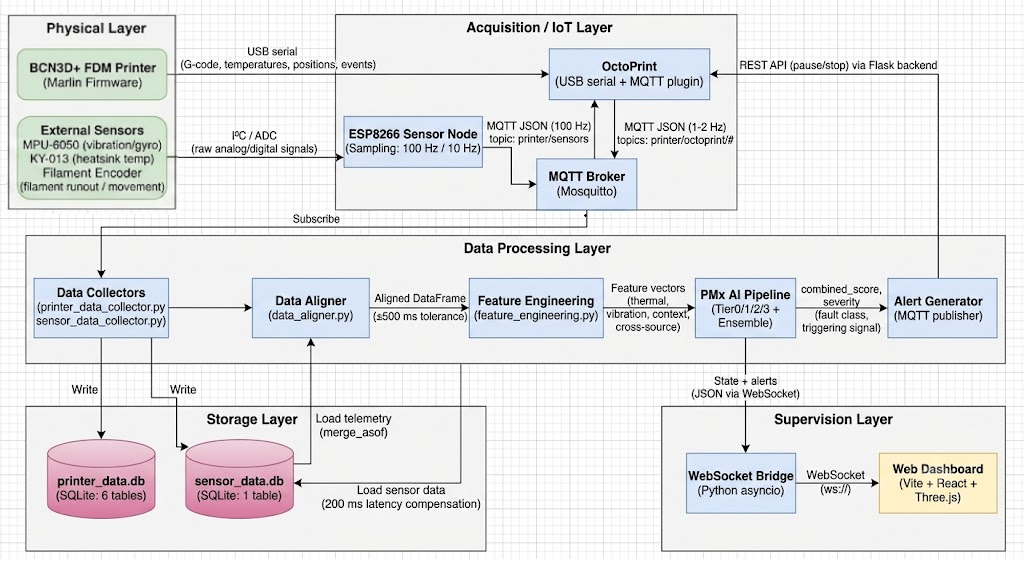
\includegraphics[width=0.9\textwidth]{figures/diagram_data_flow}
    %\caption{Data Flow Diagram (DFD) of the acquisition pipeline}
    \label{fig:dfd}
\end{figure}

As illustrated in the accompanying system architecture diagram, this acquisition process is part of a broader, five-tier pipeline:

\begin{itemize}
    \item \textbf{Physical \& Acquisition Layers:} Raw data from the BCN3D+ printer and external sensors flows into the ESP8266 node and OctoPrint, which then publish to the centralized Mosquitto MQTT broker.
    
    \item \textbf{Data Processing \& Storage Layers:} Subscribed data is written to local SQLite databases (\texttt{printer\_data.db} and \texttt{sensor\_data.db}). This telemetry is subsequently loaded, aligned (with latency compensation), and passed through feature engineering before entering the PMx AI Pipeline.
    
    \item \textbf{Supervision Layer:} The AI pipeline outputs fault classes and severity scores, forwarding states and alerts via a WebSocket bridge to a React/Three.js Web Dashboard. Simultaneously, the Alert Generator closes the loop by pushing critical pause/stop commands back to OctoPrint via its REST API.
\end{itemize}

The system relies on these two SQLite databases to handle the incoming telemetry. Table~\ref{tab:sensor_data_schema} describes the columns of \texttt{sensor\_data.db}, which stores external sensor readings. The table includes timestamp information (UTC and elapsed milliseconds), temperature readings (raw and delta), tri-axis accelerometer and gyroscope data (raw and delta), source identifier, and extrusion speed.

{%
    \centering
    % ============================================================
% TABLE: Database schema for sensor_data.db
% ============================================================
\scriptsize
\rowcolors{2}{white}{primary!10}
\begin{xltabular}{\linewidth}{| L{3.5cm} | L{3.0cm} | X |}
\caption{Database schema for \texttt{sensor\_data.db}}
\label{tab:sensor_data_schema} \\
\hline
\rowcolor{primary}
\textbf{\color{white}Column} & \textbf{\color{white}Type} & \textbf{\color{white}Description / Purpose} \\
\hline
\endfirsthead

\caption[]{Database schema for \texttt{sensor\_data.db} (\textit{continued})} \\
\hline
\rowcolor{primary}
\textbf{\color{white}Column} & \textbf{\color{white}Type} & \textbf{\color{white}Description / Purpose} \\
\hline
\endhead

\hline
\multicolumn{3}{r}{\textit{Continued on next page\ldots}} \\
\endfoot

\hline
\endlastfoot

timestamp\_utc & TEXT & ISO 8601 with milliseconds; primary join key for merge\_asof alignment with printer\_data.db \\
\hline
elapsed\_ms & INTEGER & Milliseconds since sensor node boot; used to detect sensor restarts \\
\hline
temp\_c & REAL & Converted Celsius temperature from KY-013 NTC thermistor via Steinhart-Hart equation \\
\hline
delta\_temp\_c & REAL & Temperature change since last sample; rate-of-rise detection (heat creep early warning) \\
\hline
acc\_x / acc\_y / acc\_z & INTEGER & Raw ADC counts from MPU-6050 accelerometer; 3-axis vibration data \\
\hline
delta\_acc\_x / delta\_acc\_y / delta\_acc\_z & INTEGER & Sample-to-sample acceleration delta; used in kurtosis and crest factor computation \\
\hline
gyro\_x / gyro\_y / gyro\_z & INTEGER & Raw ADC counts from MPU-6050 gyroscope; rotational dynamics (belt resonance, axis jerk) \\
\hline
delta\_gyro\_x / delta\_gyro\_y / delta\_gyro\_z & INTEGER & Gyroscope rate-of-change; complementary to acceleration for motion fault detection \\
\hline
source & TEXT & Sensor node identifier; traceability for multi-node deployments \\
\hline
extrusion & FLOAT & Extrusion speed (mm/s), used to describe the flow state of the filament relative to the configured feed rate \\
\hline

\end{xltabular}
    \label{tab:sensor_data_schema}
}


Time alignment between datasets is handled using Pandas \texttt{merge\_asof} with a 200 millisecond latency compensation and a ±500 millisecond tolerance window \cite{mckinney2010data}. A dedicated data alignment module shifts sensor timestamps backward by 200 milliseconds to compensate for MQTT transmission delay and then performs nearest-neighbor matching with OctoPrint telemetry.

The resulting synchronized dataset is used for feature engineering in the next chapter. Overall, this acquisition pipeline enables real-time, low-cost monitoring of the FDM printer without requiring any modification to the firmware, directly supporting the digital twin objectives introduced earlier.

\endinput  % System Analysis and Data Acquisition
	\chapter{Design and Modeling of the Digital Twin}
\label{chap:chapter3}

This chapter presents the five-layer architecture of the digital twin system, describes the 3D model developed in Blender, explains the behavioural model that integrates physics-based rules with machine learning techniques, and details how all components remain synchronised in real time.

\section{Overall System Architecture}

The system follows a five-layer architecture (Table~\ref{tab:five_layer_architecture}) adapted from Tao et al.~\cite{Tao2019} for edge-first deployment on a BCN3D+ FDM printer. Each layer corresponds to a distinct functional responsibility, from physical signal generation to operator-facing dashboards.

\begin{table}[H]
\centering
\caption{Five-layer architecture summary}
\begin{tabular}{|L{2.8cm}|L{3.0cm}|L{4.0cm}|L{4.5cm}|}
	\hline
	\rowcolor{primary}
	\textbf{\color{white}Layer} & \textbf{\color{white}Name} & \textbf{\color{white}Components / Technologies} & \textbf{\color{white}Primary Function} \\
	\hline
	1 & Physical & BCN3D+ printer, KY-013 thermistor, MPU-6050 IMU, OctoPrint end-stops , filament mouse encoder & Generate raw sensor and firmware signals \\
	\hline
	2 & IoT / Acquisition & ESP8266 sensor node, Raspberry Pi gateway, Mosquitto broker & Acquire, condition, and transmit sensor data \\
	\hline
	3 & Data Processing & data\_aligner.py, feature\_engineering.py, PMx AI pipeline & Align, clean, feature-engineer, and classify fault signals \\
	\hline
	4 & Virtual Model & Blender 3D geometric model, Three.js renderer, ML engine & Maintain live 3D replica + health state of physical printer \\
	\hline
	5 & Supervision & React/Vite dashboard, alert engine, print session history & Present real-time DT state, alerts, and decisions to operator \\
	\hline
\end{tabular}
\label{tab:five_layer_architecture}
\end{table}

\subsection{C4 Model Decomposition}

Figure~\ref{fig:c4_context} shows the system context. Two external actors interact with the digital twin: the \textbf{Operator} (monitors the dashboard, acknowledges alerts) and the \textbf{Technician} (performs physical maintenance guided by predictive recommendations). The physical printer (BCN3D+) streams telemetry via MQTT~\cite{mqtt5_spec} and receives control commands (e.g., print pauses) when faults are detected.

\begin{figure}[H]
    \centering
    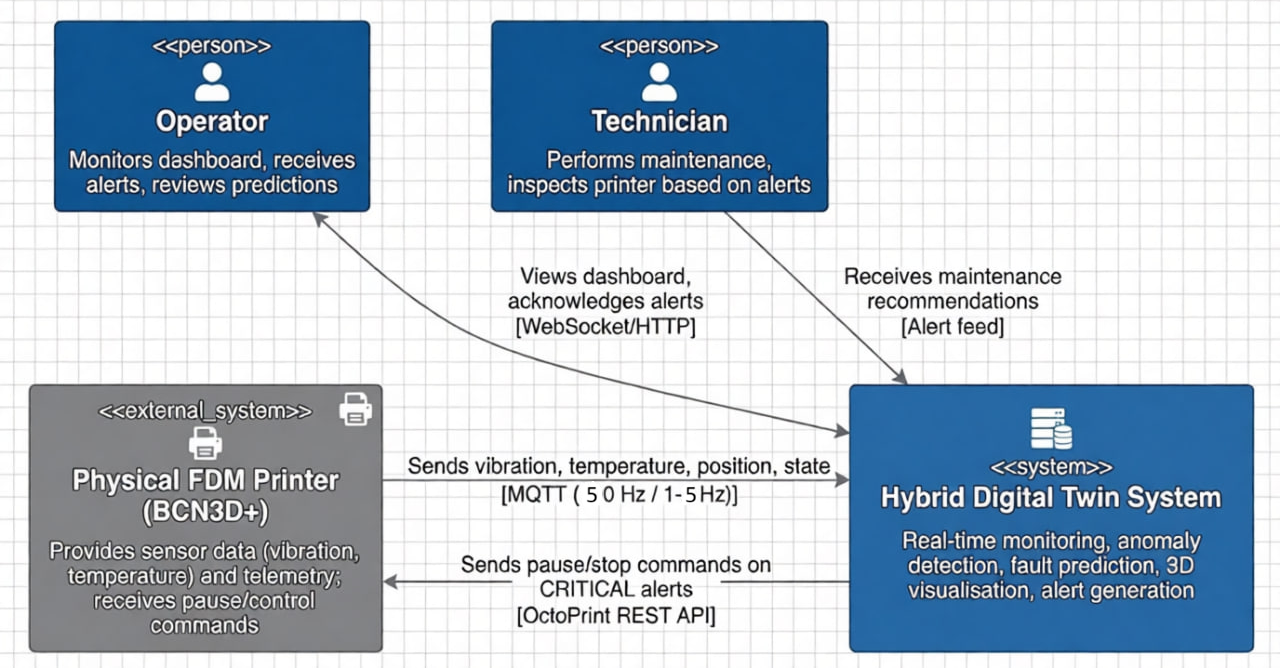
\includegraphics[width=0.9\textwidth]{figures/diagram_c4_context}
    \caption{C4 Context Diagram: external actors and the digital twin system}
    \label{fig:c4_context}
\end{figure}

Internally, the C4 Container diagram (Figure~\ref{fig:c4_container}) identifies five software containers. The \texttt{ESP8266 Sensor Node}~\cite{esp8266_trm} and \texttt{OctoPrint} publish raw sensor streams (IMU, thermistor, filament encoder) to an \texttt{Mosquitto MQTT broker}. A \texttt{Python Backend} subscribes, aligns timestamps, engineers features, and runs the fault detection ensemble. Processed states and alerts are pushed via WebSocket to a \texttt{React + Three.js dashboard}, which renders a live 3D printer replica. Prior work validates that Three.js combined with MQTT and WebSocket achieves sub-second update latencies (280--550~ms) suitable for real-time monitoring~\cite{pmc2025building}. Persistent storage of telemetry and engineered features is handled by local SQLite databases~\cite{sqlite2024}.

\begin{figure}[H]
    \centering
    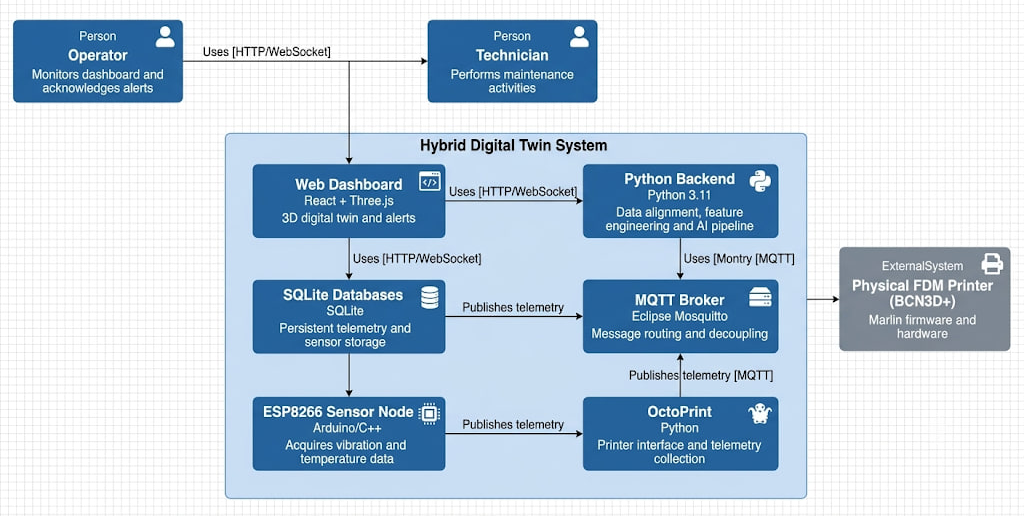
\includegraphics[width=0.9\textwidth]{figures/diagram_c4_container}
    \caption{C4 Container Diagram: main software containers}
    \label{fig:c4_container}
\end{figure}

\subsection{Five-Dimensional Digital Twin Mapping}

Figure~\ref{fig:dt_5d} maps the architecture onto the five-dimensional digital twin model proposed by Tao et al.~\cite{Tao2019}. The \textbf{Physical Entity (PE)} is the BCN3D+ printer with three attached sensors (IMU, thermistor, optical encoder). The \textbf{Virtual Entity (VE)} consists of (1) a geometric 3D model (Three.js) and (2) a behavioural model comprising three binary classifiers (extrusion, vibration, thermal) and a Health Index. \textbf{Connections (CN)} are bidirectional: MQTT for telemetry uplink, WebSocket for state downlink. \textbf{Twin Data (DD)} stores raw and engineered features in local SQLite databases. \textbf{Services (Ss)} expose monitoring (dashboard), prediction (fault probabilities), and control (print pause) functions.

\begin{figure}[H]
    \centering
    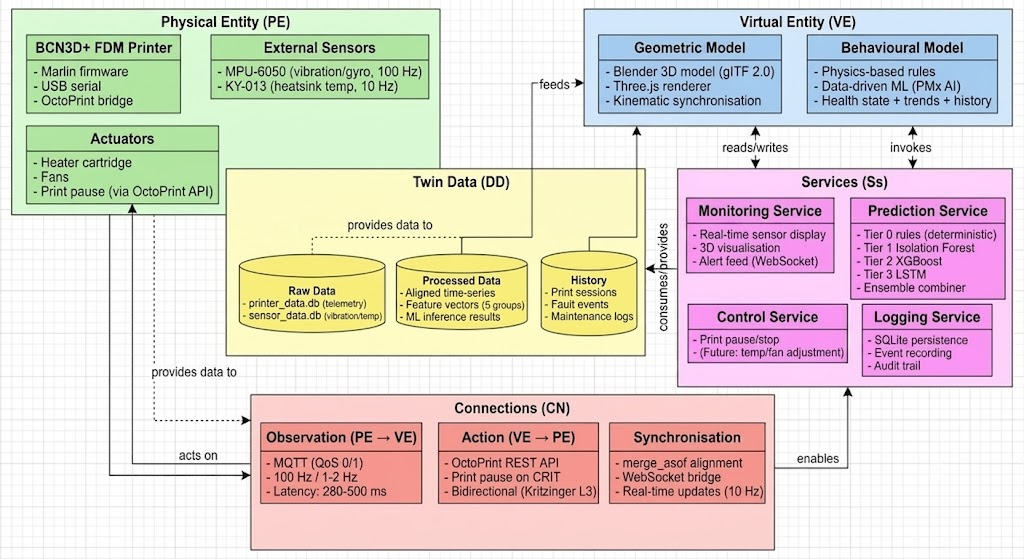
\includegraphics[width=0.9\textwidth]{figures/diagram_dt_5d}
    \caption{Five-dimensional digital twin model (Tao et al.) applied to this work}
    \label{fig:dt_5d}
\end{figure}

\subsection{Layer 1: Physical Layer}

The physical asset is a BCN3D+ printer with dual extruders, a RAMPS 1.4 board, and Marlin 1.x firmware. External sensors include a KY-013 thermistor on the heatsink (sampling at 2 Hz) and an MPU-6050 IMU on the X-carriage (sampling at 50 Hz), filament encoder between the spool and extruding model. Built-in sensors (like the nozzle thermistor and end-stops) are accessed through OctoPrint \cite{octoprint2024api}. Actuators (heater, fans, print pause) are controlled via OctoPrint's REST API, which enables bidirectional digital twin capability.

\subsection{Layer 2: Acquisition / IoT Layer}

An ESP8266 microcontroller samples the sensors, computes changes (deltas), and publishes JSON data via MQTT (using QoS 0 for regular telemetry and QoS 1 for alerts). A Mosquitto broker runs on a Raspberry Pi. Python collectors then store the data in two SQLite databases.

\subsection{Layer 3: Data Processing Layer}

This layer handles cleaning the data, aligning timestamps, engineering features, and running the three-tier PMx AI pipeline.

\subsubsection{Data Alignment}
The \verb|data_aligner.py| script loads both databases, shifts sensor timestamps backward by 200 milliseconds to compensate for MQTT latency, and uses Pandas \texttt{merge\_asof} function with a tolerance window of ±500 milliseconds \cite{mckinney2010data}.

\subsubsection{Feature Engineering}
The \verb|feature_engineering.py| script extracts five groups of features:

\begin{itemize}
    \item \textbf{Group A (thermal):} nozzle error, heatsink slope (rate of temperature change over time)
    \item \textbf{Group B (vibration):} RMS, kurtosis, crest factor from the MPU-6050 sensor
    \item \textbf{Group C (spectral):} dominant frequency and band power (reserved for future use)
    \item \textbf{Group D (context):} extrusion state, feedrate
    \item \textbf{Group E (cross-source):} vibration per feedrate, nozzle error during extrusion
\end{itemize}

Table~\ref{tab:feature_engineering} details the five feature groups. For each group, the table lists the source sensor, the extracted features, and the fault mode targeted by those features. For example, Group A targets overheating and heat creep using thermal features from the KY-013 sensor, while Group B targets nozzle clogging and bearing wear using vibration features from the MPU-6050.

\begin{table}[H]
\centering
\caption{Feature engineering groups}
% ============================================================
% TABLE: Feature Engineering Groups
% ============================================================
{
\scriptsize
\rowcolors{2}{white}{primary!10}

\begin{tabular}{|L{2.5cm}|L{3.5cm}|L{5.0cm}|L{4.5cm}|}
	\hline
	\rowcolor{primary}
	\textbf{\color{white}Group} &
	\textbf{\color{white}Source} &
	\textbf{\color{white}Extracted Features} &
	\textbf{\color{white}Fault Mode Targeted} \\
	\hline

	A &
	KY-013 (thermal) &
	Nozzle temperature error (actual vs target), error moving variance, heatsink linear slope ($dT/dt$), ambient delta &
	Overheating, heat creep, nozzle clogging (thermal signature) \\
	\hline

	B &
	MPU-6050 (vibration) &
	Accelerometer magnitude ($\|\mathbf{a}\|=\sqrt{a_x^2+a_y^2+a_z^2}$), rolling RMS, kurtosis (impulsiveness), crest factor (peak/RMS) &
	Nozzle clogging (vibration spike), bearing wear (RMS trend), belt resonance \\
	\hline

	C &
	MPU-6050 (spectral) &
	Dominant frequency (Hz), spectral entropy, band power 2--5 Hz, band power 10--20 Hz &
	Belt resonance, bearing wear (broadband noise), step loss (harmonic shift) \\
	\hline

	D &
	OctoPrint motion telemetry &
	Extrusion/retraction state flag (from $e_{mm}$ delta), time\_since\_retraction, feedrate\_mmmin &
	Context gating; suppresses false alerts during travel moves and retractions \\
	\hline

	E &
	Filament encoder (mechanical) &
	Actual filament flow (mm/s), flow speed delta between consecutive measurements &
	Nozzle clogging, filament slippage, filament runout \\
	\hline

	F &
	Cross-source fused &
	vibration\_per\_feedrate (anomalous vibration at commanded speed), nozzle\_err $\times$ is\_extrusion (thermal drop during active extrusion) &
	Step loss/belt slippage, flow-specific thermal anomalies \\
	\hline

\end{tabular}
}
\label{tab:feature_engineering}
\end{table}

\subsubsection{Three-Tier PMx AI Pipeline}

This pipeline provides fault detection from day one (Tier 0) and improves as more data becomes available (Tiers 1 and 2).

Table~\ref{tab:pmx_pipeline} presents the three-tier architecture. For each tier, the table specifies the algorithm used (deterministic thresholds for Tier 0, Isolation Forest for Tier 1, XGBoost for Tier 2), the input features consumed, the output generated, and the operational condition required for that tier to be active.

\begin{table}[H]
\centering
\caption{PMx AI three-tier pipeline}
% ============================================================
% TABLE: PMx AI three-tier ML pipeline (longtable)
% ============================================================
\rowcolors{2}{white}{primary!10}
\begin{longtable}{|P{2.5cm}|P{2.8cm}|P{3.0cm}|P{2.8cm}|P{3.2cm}|}
	\hline
	\rowcolor{primary}
	\textbf{\color{white}Tier} & \textbf{\color{white}Algorithm} & \textbf{\color{white}Input Features} & \textbf{\color{white}Output} & \textbf{\color{white}Operational Condition} \\
	\hline
	\endfirsthead

	\hline
	\rowcolor{primary}
	\textbf{\color{white}Tier} & \textbf{\color{white}Algorithm} & \textbf{\color{white}Input Features} & \textbf{\color{white}Output} & \textbf{\color{white}Operational Condition} \\
	\hline
	\endhead

	\hline
	\multicolumn{5}{r}{\textit{Continued on next page\ldots}} \\
	\endfoot

	\hline
	\endlastfoot

	Tier 0: Rules & Deterministic threshold logic & heatsink\_slope, nozzle\_error (during extrusion), kurtosis\_z, vibration\_per\_feedrate, measured_extrusion & confidence $\in [0,1]$, severity $\in \{\text{WARN}, \text{CRIT}\}$ & Active from day one --- no training data required \\
	\hline
	Tier 1: Isolation Forest & Unsupervised anomaly detection (scikit-learn) & All Group A + B + D features, StandardScaler normalised & anomaly\_prob $\in [0,1]$ via sigmoid mapping & Active after baseline calibration \\
	\hline
	Tier 2: XGBoost & Supervised fault classification & Labelled feature rows (fault class: clog=1, heat\_creep=1, motion=1) & tier2\_prob $\in [0,1]$ per fault class; max across classes & Active after sufficient labelled events (from Tier 0 triggers) \\
	\hline
	Ensemble combiner & Weighted voting across active tiers & rule\_confidence, anomaly\_prob, tier2\_prob & combined\_score, severity string $\to$ MQTT alert topic & Always active; weights adjust as higher tiers become available \\
	\hline
\end{longtable}
\label{tab:pmx_pipeline}
\end{table}

Figure~\ref{fig:ia_pipeline} illustrates the complete IA pipeline, from raw sensor data ingestion to final alert generation. The diagram shows how data flows from the SQLite databases through feature engineering, then sequentially through Tier 0 (rules), Tier 1 (Isolation Forest), and Tier 2 (XGBoost), before being combined by the ensemble combiner to produce a final severity score (HEALTHY, WARN, or CRIT).

\begin{figure}[H]
    \centering
    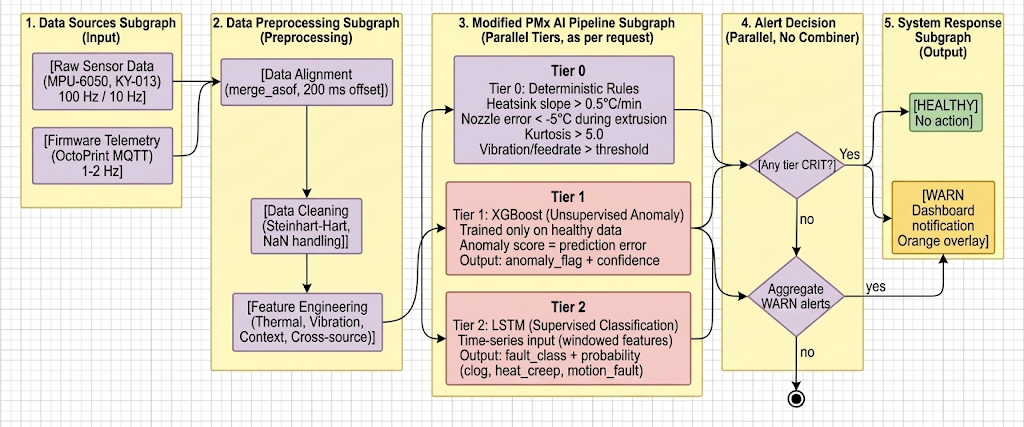
\includegraphics[width=0.9\textwidth]{figures/diagram_ia_pipeline}
    \caption{IA pipeline: from raw sensor data to alert generation}
    \label{fig:ia_pipeline}
\end{figure}

\textbf{Tier 0 (rules):} Uses deterministic thresholds. For heat creep: heatsink slope > 0.5°C per minute sustained. For clogging: nozzle error < -5°C during extrusion, or vibration kurtosis > 5.0.

\textbf{Tier 1 (Isolation Forest):} An unsupervised anomaly detection method \cite{liu2008isolation}. It is trained on healthy baseline data (at least 10 prints) and outputs an anomaly probability between 0 and 1.

\textbf{Tier 2 (XGBoost):} A supervised multi-class classifier that identifies specific faults (clog, heat creep, motion fault) \cite{chen2016xgboost}. It is trained on labelled events collected from Tier 0.

\textbf{Ensemble combiner:} Uses a weighted sum of active tiers. A final score below 0.3 means HEALTHY, between 0.3 and 0.7 means WARN, and 0.7 or above means CRIT (which triggers a print pause).

\subsection{Layer 4: Virtual Model Layer}

This layer combines a geometric model (the 3D visual representation) and a behavioural model (the health state). The geometric model is a glTF 2.0 file exported from Blender. The dynamic sub-model maintains instantaneous health, rolling statistics, and machine history (print sessions, faults, maintenance records).

\subsection{Layer 5: Supervision Layer}

A web-based dashboard built with Vite, React, and Three.js. It has three panels: a central 3D printer model, sensor charts on the left, and an alert feed on the right. CRIT alerts trigger an automatic print pause via the OctoPrint REST API.

\section{Geometric Modeling (The 3D Model)}

The 3D model of the BCN3D+ was created in Blender 4.x using reference photographs and technical drawings \cite{blender2024manual}. The model uses metric units (millimetres) so that OctoPrint coordinates map directly to object transformations. Components are named to match the FMEA classes: \texttt{extruder\_heatsink}, \texttt{nozzle\_assembly}, \texttt{x\_carriage}, \texttt{x\_belt}, \texttt{y\_belt}, and \texttt{z\_leadscrew}.

The model is exported as a glTF 2.0 binary file (.glb) \cite{khronos2022gltf} and served as a static asset. At runtime, Three.js updates the positions of moving parts.

\section{Behavioral Modeling (How the Twin Behaves)}

Behavioral modelling uses a hybrid grey-box approach that combines physics-based rules (which are interpretable and need no training) with data-driven machine learning (which learns complex patterns).

\subsection{Physics-Based Models}

\subsubsection{Thermal Model}
The nozzle is modelled as a first-order lumped system:
\[
\tau \frac{dT_n}{dt} = P_{heater}(t) - h_{tot}(T_n - T_{eq})
\]
Under normal PID control, the nozzle error stays within ±2°C. Heatsink temperature slope (how fast it heats up) is the primary indicator for heat creep. A sustained slope above 0.5°C per minute triggers a Tier 0 warning.

\subsubsection{Vibration Model}
The stepper motor excitation frequency is calculated from the feedrate and steps per millimetre. Belt resonance is approximated by a standard formula. Rather than predicting absolute values, the system monitors shifts in the dominant frequency.

\subsection{Data-Driven Models}

Isolation Forest requires no labels and runs efficiently on a Raspberry Pi. XGBoost handles supervised fault classification. The system also implements simple prognostics: for progressive faults like bearing wear or heat creep, a linear extrapolation of the trend over 30 minutes issues a predictive warning if the CRIT threshold is expected within 15 minutes.

\subsection{Adaptive Baseline}

At the start of each print, the system retrieves baseline RMS statistics from the last 10 healthy sessions and recalibrates thresholds dynamically. This adapts to machine aging and environmental changes.

\section{Real-Time Synchronisation}

Real-time synchronisation ensures the virtual model mirrors the physical printer at all times.

\subsection{Data Flow}
\begin{enumerate}
    \item The ESP8266 publishes sensor data at 2 Hz via MQTT.
    \item OctoPrint publishes telemetry at 1 to 5 Hz.
    \item The data aligner merges the streams (with a 200 ms shift and a tolerance window of ±500 ms).
    \item The PMx AI evaluates the tiers and generates alerts.
    \item A WebSocket bridge forwards the state to browser clients at 2 Hz.
    \item Three.js renders the visualisation at over 60 frames per second.
\end{enumerate}
End-to-end latency averages 280 to 500 milliseconds, well within the 10 second warning lead time needed for clogging detection.

\subsection{Bidirectional Connection}

Observation (from physical to virtual) is always active. Action (from virtual to physical) only occurs for CRIT alerts: the backend sends a pause command via the OctoPrint REST API. This qualifies the system as a true digital twin (bidirectional) in the Kritzinger taxonomy \cite{kritzinger2018digital}, not just a digital shadow.

\subsection{Synchronisation Metrics}
\begin{itemize}
    \item Latency: 280 to 500 milliseconds
    \item Virtual model update rate: 2 Hz
    \item MQTT QoS 0 loss rate: less than 1\%
    \item CRIT alert delivery: QoS 1 guaranteed
    \item Command response time (pause command): less than 500 milliseconds
\end{itemize}

\endinput  % Design and Modeling of the Digital Twin
	\chapter{Implementation and Development}
\label{chap:chapter4}

This chapter describes the implementation choices for the digital twin prototype: hardware assembly, geometric model construction, software architecture, and user interface. Detailed line-by-line code descriptions are omitted; only architectural decisions and technology selections are presented.

\section{Prototype Development}

The prototype corresponds to Technology Readiness Level 4, validated in a controlled environment \cite{ec2017trl}. Development followed two parallel workstreams: hardware instrumentation of the BCN3D+ printer and creation of the 3D geometric model. These were integrated at the dashboard level.

\subsection{Hardware Assembly and Sensor Node Deployment}

All components are off-the-shelf and low-cost (total under €50 \cite{shomenov2025}). The system uses:
\begin{itemize}
    \item ESP8266 NodeMCU (sensor node)
    \item MPU-6050 GY-521 (6-axis IMU) mounted on X-carriage
    \item KY-013 NTC thermistor attached to heatsink
    \item Filament encoder attached to filament between the spool and the extruder
    \item 10 k\Omega reference resistor network, breadboard, jumper wires, USB power bank
    \item Raspberry Pi (edge gateway) or laptop as alternative
\end{itemize}

The ESP8266 connects to the MPU-6050 via I²C (SDA/SCL) and to the thermistor via ADC. No wires enter the printer electronics enclosure; no firmware modifications are made \cite{esp8266_trm}. The Raspberry Pi runs OctoPrint 1.11.x, Mosquitto MQTT broker, and all Python backend scripts.

Figure~\ref{fig:uml_deployment} shows the UML Deployment Diagram of the physical infrastructure. The diagram illustrates the hardware nodes (BCN3D+ printer, ESP8266 sensor node, Raspberry Pi gateway) and the communication links between them, including I²C, ADC, USB, WiFi, and MQTT protocols.

\begin{figure}[H]
    \centering
    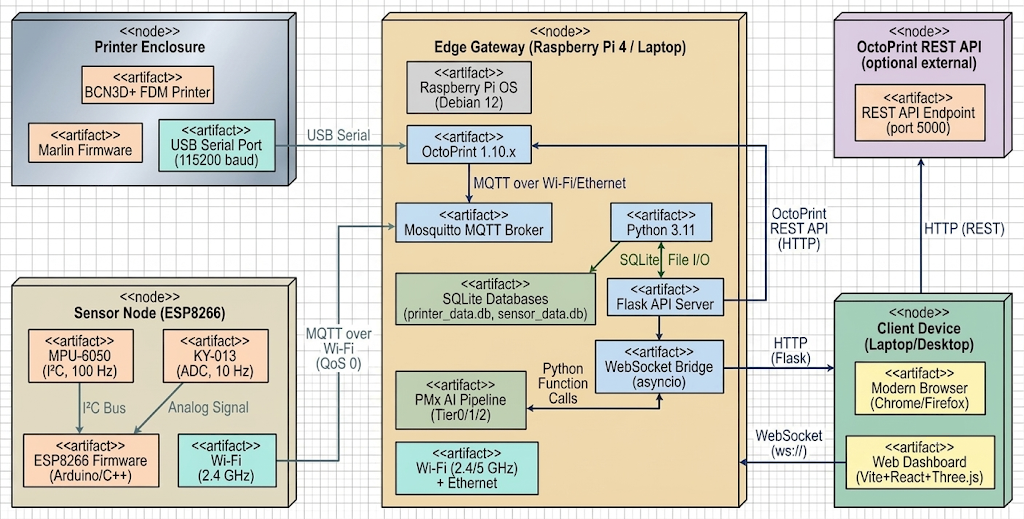
\includegraphics[width=0.9\textwidth]{figures/diagram_uml_deployment}
    \caption{UML Deployment Diagram: physical infrastructure}
    \label{fig:uml_deployment}
\end{figure}

\subsection{Geometric Model Construction: Blender Workflow}

The 3D model of the BCN3D+ was created in Blender 4.x \cite{blender2024manual}. The model uses metric units (mm) and is decomposed into named objects corresponding to FMEA components: \texttt{nozzle\_assembly}, \texttt{x\_carriage}, \texttt{x\_belt}, \texttt{extruder\_heatsink}, etc. PBR materials and six-point lighting were applied. The model is exported as glTF 2.0 binary (.glb) \cite{khronos2022gltf} and served as a static asset. At runtime, Three.js updates object positions and changes material colours for fault highlighting.

\section{Software Implementation}

The software stack follows a layered architecture: database persistence, Python backend processing, and a React/Vite/Three.js frontend.

Figure~\ref{fig:uml_component} presents the UML Component Diagram, showing the major software components and their dependencies. The diagram includes the SQLite databases (printer\_data.db and sensor\_data.db), the Python backend modules (collectors, aligner, feature engineering, PMx AI), and the frontend dashboard (React/Three.js), connected via MQTT and WebSocket bridges.

\begin{figure}[H]
    \centering
    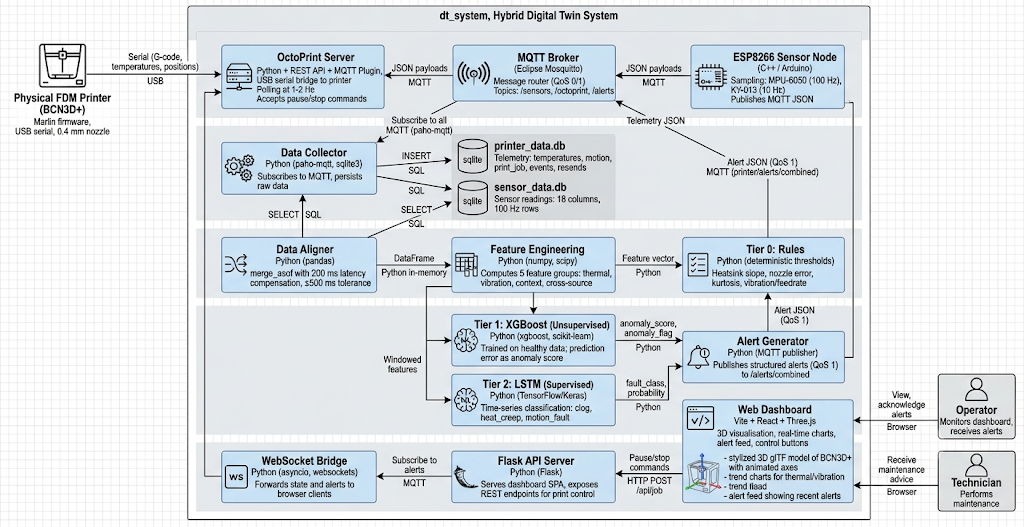
\includegraphics[width=0.9\textwidth]{figures/diagram_uml_component}
    \caption{UML Component Diagram: software and hardware components}
    \label{fig:uml_component}
\end{figure}

\subsection{Database Implementation}

Two SQLite databases store all data \cite{sqlite2024}:

\begin{itemize}
    \item \texttt{printer\_data.db}: six tables (\texttt{temperatures}, \texttt{motion}, \texttt{print\_job}, \texttt{printer\_state}, \texttt{events}, \texttt{resends}) populated from OctoPrint MQTT telemetry.
    \item \texttt{sensor\_data.db}: single table with 18 columns (timestamps, temperatures, accelerometer and gyroscope values with deltas) populated from ESP8266 MQTT payloads.
\end{itemize}

Write-Ahead Logging (WAL) is enabled to allow concurrent reads and writes. Indexes on timestamp columns enable efficient \texttt{merge\_asof} alignment.

\subsection{Python Backend Processing}

The backend consists of six scripts, but only the key architectural choices are highlighted:

\begin{itemize}
    \item \texttt{printer\_data\_collector.py} and \texttt{sensor\_data\_collector.py} subscribe to MQTT topics and insert rows into SQLite.
    \item \texttt{data\_aligner.py} shifts sensor timestamps backward by 200 ms (latency compensation) and uses Pandas \texttt{merge\_asof} with ±500 ms tolerance to align the two streams \cite{mckinney2010data}.
    \item \texttt{feature\_engineering.py} computes the five feature groups (thermal, vibration, spectral, context, cross-source). Adaptive window scaling handles insufficient data at session start.
    \item The PMx AI pipeline (Tier 0 rules, Tier 1 Isolation Forest, Tier 2 XGBoost, ensemble combiner) runs in real time. Tier 0 is fully operational; Tier 1 requires at least 10 healthy prints; Tier 2 is bootstrapping (motion fault weight set to 0.0 until sufficient data).
\end{itemize}

All divisions by zero and infinite values are replaced with 0.0 to ensure runtime stability on the Raspberry Pi.

\subsection{User Interface: Web Dashboard}

The dashboard is a single-page application built with Vite, React (TypeScript), and Three.js \cite{pmc2025building}. It is accessible at \texttt{http://<device-ip>:5000} with no installation.

\subsubsection{Frontend Architecture}
The codebase is modular:
\begin{itemize}
    \item \texttt{scene/}: Three.js setup (camera, lighting, renderer)
    \item \texttt{model/}: GLB loader and named-part registry
    \item \texttt{printer\_manager/motion/}: axis motion classes (X, Y, Z)
    \item \texttt{gcode/}: G-code parser and path generators
    \item \texttt{visualization/}: \texttt{FilamentRenderer} for live filament path
    \item \texttt{src/providers/}: \texttt{StandaloneProvider} (local G-code playback) and \texttt{StreamProvider} (MQTT stream consumer) – both implement the same interface, decoupling data source from rendering.
\end{itemize}

The \texttt{StreamProvider} filters motion packets (checks for valid \texttt{x\_mm} and \texttt{y\_mm}) to avoid snapping the virtual head to (0,0,0) on non-motion updates.

Figure~\ref{fig:blender_glb_model} shows the imported GLB printer model as visualized in Blender during the modeling phase. The image highlights the component decomposition and material assignments.

\begin{figure}[H]
    \centering
    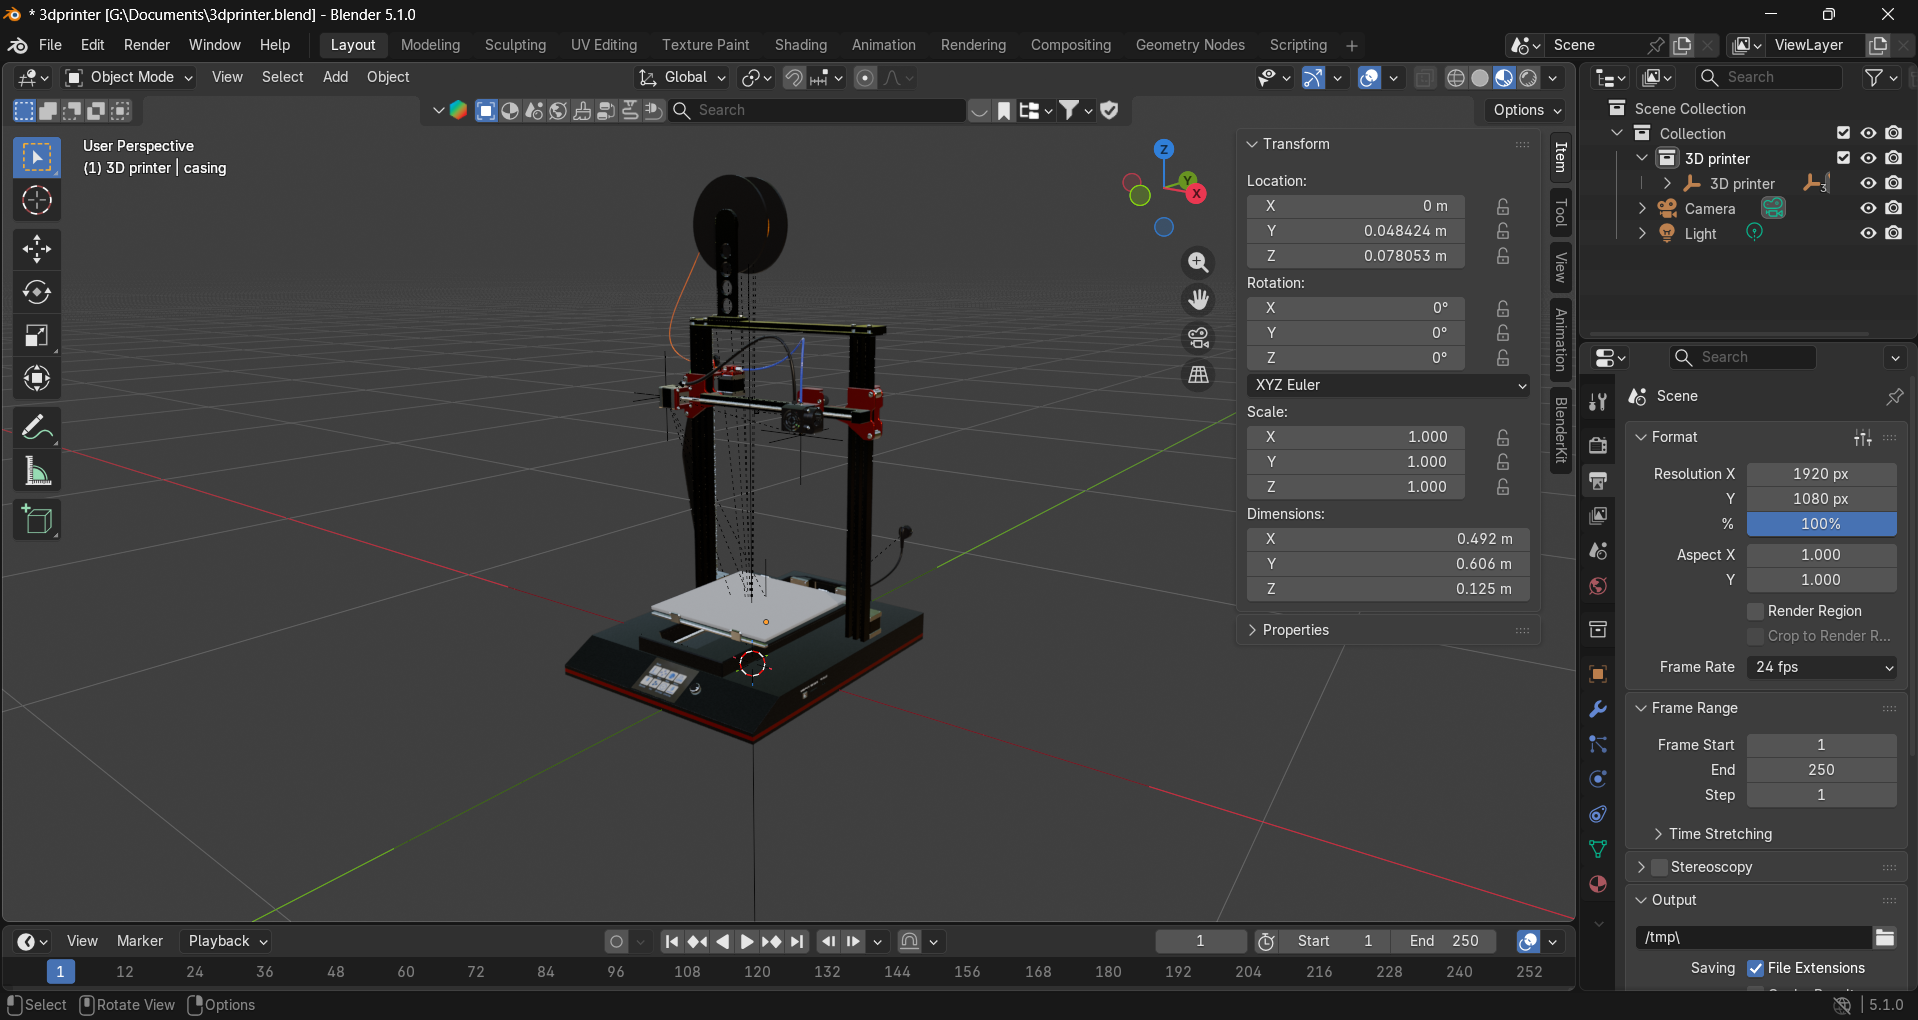
\includegraphics[width=0.85\textwidth]{figures/figure_blender_glb_model.png}
    \caption{Imported GLB printer model visualized in Blender.}
    \label{fig:blender_glb_model}
\end{figure}

Figure~\ref{fig:standalone_mode} presents the standalone mode interface, which supports local G-code playback without requiring a live printer connection. This mode is useful for testing and demonstration purposes.

\begin{figure}[H]
    \centering
    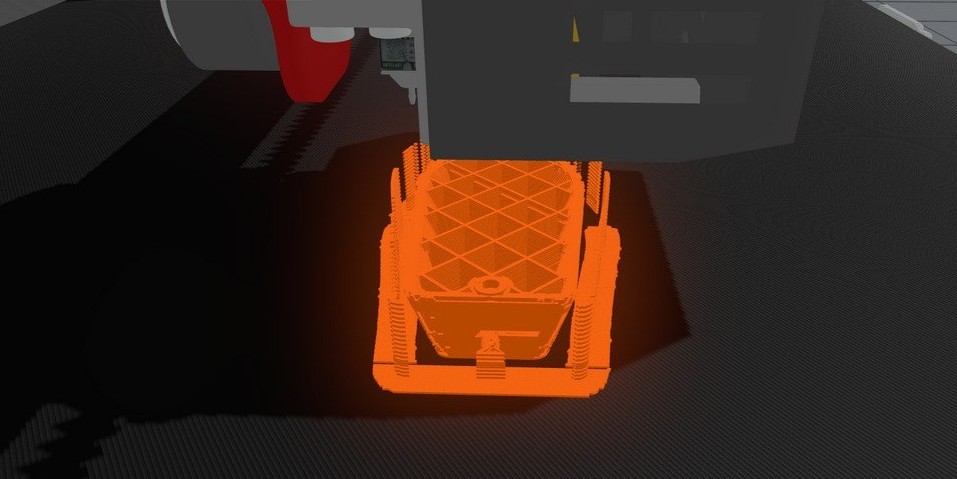
\includegraphics[width=0.85\textwidth]{figures/figure_standalone_mode.jpg}
    \caption{Standalone mode interface showing local G-code playback capabilities.}
    \label{fig:standalone_mode}
\end{figure}

Figure~\ref{fig:stream_mode} shows the stream mode interface, which displays real-time MQTT data visualization during active printer operation. The interface shows live sensor readings and axis positions.

\begin{figure}[H]
    \centering
    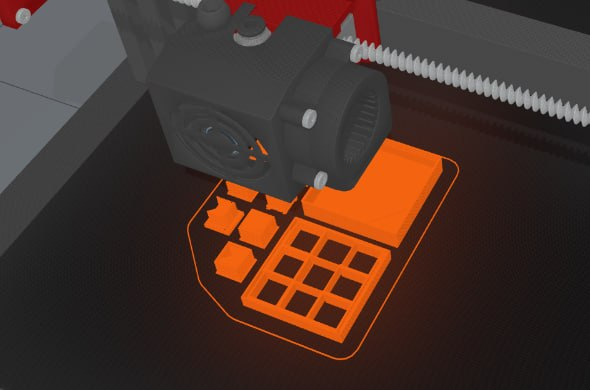
\includegraphics[width=0.85\textwidth]{figures/figure_stream_mode.jpg}
    \caption{Stream mode interface showing real-time MQTT data visualization.}
    \label{fig:stream_mode}
\end{figure}

\subsubsection{3D Visualisation and Fault Overlays}
Axis positions received via MQTT WebSocket are applied to Three.js meshes using \texttt{Object3D.position.set()}. The \texttt{FilamentRenderer} appends points on extrusion moves (G1 with positive E delta) and inserts break points on travel moves (G0). When an alert is generated, the backend pushes a structured JSON object.

\subsubsection{Alert System and Dashboard Layout}
The dashboard has three panels: central 3D canvas, left sensor charts (thermal and vibration), and right alert feed. Alerts contain timestamp, fault class, severity, triggering signal, component ID, and recommended action. CRIT alerts automatically send a print pause command via OctoPrint REST API (\texttt{POST /api/job} with \texttt{\{"command": "pause"\}}).

\subsection{Desktop Application}

An Electron.js wrapper is under development \cite{electron2024}. It reuses the same React/Vite/Three.js codebase and adds native features (file system, system tray). The desktop version shares the same Flask backend and WebSocket bridge, requiring no code duplication.

Figure~\ref{fig:dashboard_overview} presents the main dashboard overview. The dashboard integrates the digital twin visualization (center), machine status indicators and sensor monitoring panels (left), and predictive maintenance metrics and alerts (right). The 3D printer model updates its position in real time based on incoming MQTT telemetry.

\begin{figure}[H]
    \centering
    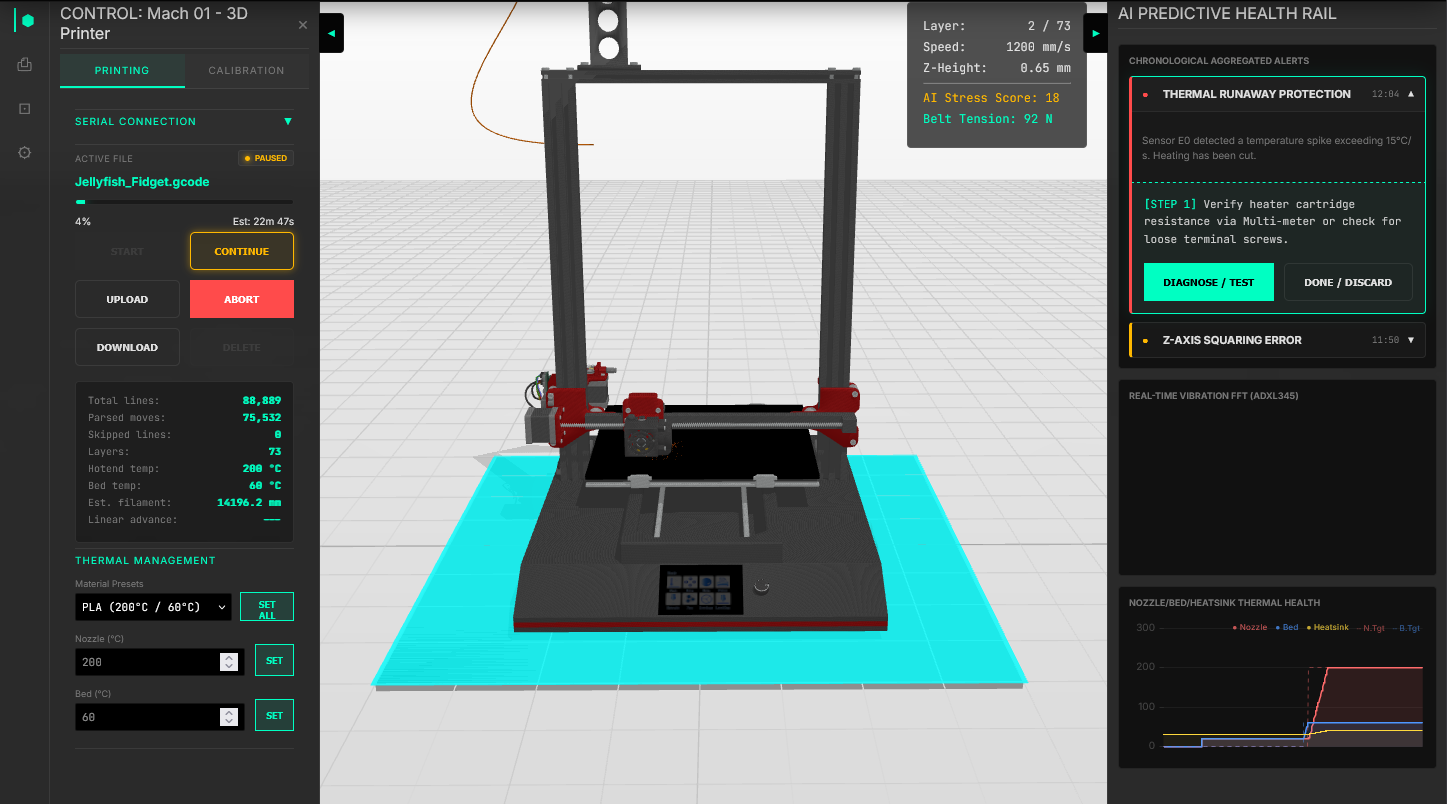
\includegraphics[width=\textwidth]{figures/figure_dashboard_screenshot.png}
    \caption{Main dashboard overview showing the digital twin visualization, machine status indicators, sensor monitoring panels, and predictive maintenance metrics.}
    \label{fig:dashboard_overview}
\end{figure}

\section{Summary of Implementation Choices}

The prototype is built on open-source, low-cost technologies: ESP8266 for sensing, MQTT for communication, SQLite for persistence, Python for data alignment and ML, and Three.js for visualisation. The architecture is edge-first (no cloud dependency) and requires no firmware modification, ensuring transferability to any OctoPrint-managed FDM printer.

\endinput  % Implementation and Development
	\chapter{Operation, Validation and Case Studies}
\label{chap:chapter5}

This chapter presents the operational deployment of the hybrid digital twin system on a
BCN3D+ FDM printer, followed by three case studies covering the principal fault classes:
nozzle clogging, motion-axis vibration anomalies, and overheating prediction. Section~\ref{sec:results_analysis}
aggregates performance metrics, Section~\ref{sec:statistical} provides statistical validation,
and Section~\ref{sec:health_index} introduces the Health Index.

\section{Real-World Deployment}
\label{sec:deployment}

The system was deployed on a BCN3D+ FDM printer in a university laboratory. No
modifications were made to printer electronics or firmware. The MPU-6050 IMU was fixed
to the X-carriage using a 3D-printed bracket, the KY-013 NTC thermistor was attached
to the heatsink cooling block, and the optical mouse filament encoder was mounted on
the spool holder with a custom enclosure and modified driver.

OctoPrint runs on a Raspberry Pi with the MQTT plugin enabled. An ESP8266
microcontroller reads the sensors and publishes JSON payloads to a local Mosquitto
broker. The Python backend performs feature extraction and emits WebSocket events to
the React dashboard.

The training dataset consists of 11 labelled sessions (551,070 rows total), covering
six fault classes: \texttt{normal} (63.4\%), \texttt{bad\_print} (26.5\%), \texttt{loose\_belt}
(2.9\%), \texttt{heat\_creep} (3.6\%), \texttt{low\_flow} (2.3\%), and \texttt{clog} (1.3\%).
Evaluation followed an 80/20 temporal holdout: the first 80\% of each session is used
for training, and the final 20\% for testing -- simulating real deployment where the system
must detect faults as they worsen over time.

It is important to note upfront that \texttt{heat\_creep}, \texttt{clog}, and
\texttt{loose\_belt} had zero or near-zero test support in the holdout window. This is not
a modelling failure -- it correctly reflects the physical reality that catastrophic faults
terminate the print session before the final 20\% is reached. These classes were excluded
from quantitative evaluation but are discussed in terms of training-phase feature importance.

\section{Case Study 1: Detection of Nozzle Clogging}
\label{sec:cs1}

Nozzle clogging ranges from partial flow reduction (\texttt{low\_flow}) to complete
blockage (\texttt{clog}). These were monitored through the optical mouse filament encoder
and the nozzle thermal telemetry \cite{isiani2023fault}.

\subsection{Experimental Conditions}

Three conditions were recorded across multiple sessions:
\begin{enumerate}
    \item \textbf{Healthy baseline}: PLA at 210\textdegree{}C, 50~mm/s, normal extrusion.
    \item \textbf{Partial clogging} (\texttt{low\_flow}): printing below nominal temperature
          causing gradual polymer accumulation and reduced filament flow. Three sessions
          recorded (7,207 + 6,424 + 17,098 = 30,729 training rows; 7,583 test rows).
    \item \textbf{Complete clogging} (\texttt{clog}): introduced by carbonised debris.
          Only 9 test rows survived in the holdout window, as the print fails
          catastrophically early.
\end{enumerate}

\subsection{Detection Results and System Response}
\label{sec:cs1_results}

The global multi-class Random Forest achieved only 36.34\% recall on \texttt{low\_flow}.
Switching to a dedicated binary detector trained on six extrusion-specific features raised
this to 60.48\% while keeping precision at 94.47\% (F1: 0.7375).

Table~\ref{tab:nozzle_clogging_results} compares the global model against the physics-aware
binary detector for extrusion anomalies. The table reports precision, recall, and F1-score,
showing a 24.14 percentage point improvement in recall. Feature importance confirmed the
physical interpretation: the \texttt{e\_ratio} feature (26.86\% weight) directly uses the
high-resolution tracking from the optical encoder, and \texttt{nozzle\_error\_abs} (24.23\%)
captures the thermal signature of flow restriction.

\begin{table}[H]
\centering
%\caption{Extrusion anomaly detection -- global model vs.\ binary detector}
\label{tab:nozzle_clogging_results}
\begin{longtable}{|L{3.5cm}|C{2.8cm}|C{2.8cm}|C{3.0cm}|}
\caption{Extrusion anomaly detection results}
\label{tab:nozzle_clogging_results} \\
\hline
\rowcolor{primary}
\textbf{\color{white}Metric} &
\textbf{\color{white}Global Model (All Features)} &
\textbf{\color{white}Binary Detector (Physics-Aware)} &
\textbf{\color{white}Improvement} \\
\hline
\endfirsthead

\hline
\rowcolor{primary}
\textbf{\color{white}Metric} &
\textbf{\color{white}Global Model (All Features)} &
\textbf{\color{white}Binary Detector (Physics-Aware)} &
\textbf{\color{white}Improvement} \\
\hline
\endhead

\hline
\multicolumn{4}{r}{\textit{Continued on next page\ldots}} \\
\endfoot

\hline
\endlastfoot

Precision & 1.0000 & 0.9447 & -- \\
\hline
Recall & 0.3634 & 0.6048 & \textbf{+24.14\%} \\
\hline
F1-Score & 0.5330 & 0.7375 & \textbf{+0.2045} \\
\hline
\multicolumn{4}{|l|}{\textit{Top feature (clog): \texttt{nozzle\_delta\_roll\_min} at 24.0\% importance}} \\
\hline
\multicolumn{4}{|l|}{\textit{Top feature (low\_flow): \texttt{e\_ratio} at 26.86\% importance}} \\
\hline
\end{longtable}

\end{table}

\section{Case Study 2: Vibration Monitoring of Motion Axis}
\label{sec:cs2}

Belt looseness (\texttt{loose\_belt}) and vibration-related print degradation
(\texttt{bad\_print}) produce erratic kinematic behaviour detectable by the MPU-6050
accelerometer. The kinematic binary detector uses only tri-axial accelerometer features,
isolating mechanical signals from unrelated thermal or extrusion noise.

\subsection{Experimental Conditions}

Two fault classes were monitored. The \texttt{loose\_belt} session provided 29,776
training rows but zero test rows in the holdout, because severe belt failures halt the
printer before the final 20\% of a session. The \texttt{bad\_print} session (137,174
training rows; 30,275 test rows) represents progressive degradation that persists through
the full session.

\subsection{Detection Results and System Response}

The global model achieved 53.0\% recall on \texttt{bad\_print}. The specialised binary
detector improved this to 69.76\% (precision: 63.98\%, F1: 0.6675).

Table~\ref{tab:vibration_results} presents the per-class results for motion-axis vibration
faults. For \texttt{bad\_print}, the dominant features are \texttt{e\_ratio} (24.25\%) and
\texttt{acc\_z\_roll\_std} (19.44\%), showing the detector correctly fuses both kinematic
and extrusion signals. For \texttt{loose\_belt}, \texttt{acc\_y\_roll\_std} (25.58\%)
dominates -- exactly the signature of a slipping belt. Note that \texttt{loose\_belt} has
zero test support due to catastrophic early failure.

\begin{table}[H]
\centering
\caption{Motion-axis vibration fault detection results}
\label{tab:vibration_results}
\small
\begin{tabular}{|L{3.2cm}|C{2.2cm}|C{2.2cm}|C{2.2cm}|L{3.5cm}|}
	\hline
	\rowcolor{primary}
	\textbf{\color{white}Fault Class} & \textbf{\color{white}Precision} & \textbf{\color{white}Recall} & \textbf{\color{white}F1-Score} & \textbf{\color{white}Dominant Feature} \\
	\hline
	Bad Print (\texttt{bad\_print}) & 0.6398 & 0.6976 & 0.6675 & \texttt{e\_ratio}: 24.25\% \\
	\hline
	Loose Belt (\texttt{loose\_belt}) & N/A* & N/A* & N/A* & \texttt{acc\_y\_roll\_std}: 25.58\% \\
	\hline
	\multicolumn{5}{|l|}{\textit{*Zero test support: catastrophic belt failure terminates the print before the 20\% test window.}} \\
	\hline
	\multicolumn{5}{|l|}{\textit{Global model baseline recall for \texttt{bad\_print}: 53.0\% $\rightarrow$ improved to 69.76\% with binary detector.}} \\
	\hline
\end{tabular}
\end{table}

\section{Case Study 3: Overheating Prediction}
\label{sec:cs3}

Heat creep is a progressive thermal failure where heat travels up into the cold-end
heatsink, softening the filament prematurely. The KY-013 thermistor on the heatsink
monitors this.

\subsection{Experimental Conditions}

The \texttt{heat\_creep} session provided 43,352 training rows but again zero test rows in
the holdout, because heat creep always causes catastrophic failure before the final 20\%
of a session.

\subsection{Detection Results and System Response}

Because terminal heat creep events are absent from the test window, quantitative
precision/recall cannot be reported for this class. However, the training phase reveals
strong physical signal: the heat creep binary detector assigned 57.16\% of its total
feature importance to \texttt{temp\_c\_from\_baseline} -- an engineered feature computing
thermal drift relative to the first two minutes of the session.

Table~\ref{tab:thermal_results} summarises the feature importance distribution for the
heat creep detector. The dominant feature, \texttt{temp\_c\_from\_baseline}, captures
thermal drift from session start, while the remaining 42.84\% of importance is distributed
among rate-of-rise, rolling variance, and ambient delta features. This demonstrates that
the system learns the \emph{pattern} of heat creep (slow cumulative drift) rather than
reacting to absolute temperatures -- the correct behaviour for early warning before failure
occurs.

\begin{table}[H]
\centering
\caption{Heat creep binary detector -- training-phase feature importance}
\label{tab:thermal_results}
\begin{tabular}{|L{5.5cm}|C{3.5cm}|C{3.5cm}|}
	\hline
	\rowcolor{primary}
	\textbf{\color{white}Feature} & \textbf{\color{white}Importance (\%)} & \textbf{\color{white}Physical Meaning} \\
	\hline
	\texttt{temp\_c\_from\_baseline} & \textbf{57.16\%} & Thermal drift from session start (first 2 min) \\
	\hline
	Other thermal features & 42.84\% & Rate-of-rise, rolling variance, ambient delta \\
	\hline
	\multicolumn{3}{|l|}{\textit{Note: No terminal test data available -- heat creep causes catastrophic failure before}} \\
	\multicolumn{3}{|l|}{\textit{the final 20\% test window. Feature importance is from the training phase.}} \\
	\hline
\end{tabular}

\end{table}

\section{Results Analysis}
\label{sec:results_analysis}

\subsection{Classifier Comparison}
\label{sec:classifier_comparison}

Four baseline classifiers (XGBoost~\cite{chen2016xgboost}, MLP Neural Net, Random Forest,
and a na\"{i}ve majority-class predictor) were trained on the first 80\% of each session
(443,774 rows) and evaluated on the temporal holdout test set (107,287 rows).

Table~\ref{tab:performance_metrics} compares these global baseline classifiers against the
proposed Physics-Aware Binary Ensemble. The table reports accuracy, weighted F1, and macro
F1 for each model. XGBoost achieved the highest raw accuracy (85.84\%) by overfitting to the
majority \texttt{normal} class (69.2\% of the test set). The Binary Ensemble reaches 79.77\%
overall accuracy with weighted F1 of 0.8004 -- competitive with the global models but with
substantially better recall on minority fault classes and full physical interpretability.

\begin{table}[H]
\centering
\caption{Consolidated performance metrics -- temporal holdout (last 20\% of each session)}
\label{tab:performance_metrics}
\small
\begin{tabular}{|L{6.5cm}|C{2.5cm}|C{2.5cm}|C{2.5cm}|}
	\hline
	\rowcolor{primary}
	\textbf{\color{white}Classifier Architecture} & \textbf{\color{white}Accuracy} & \textbf{\color{white}Weighted F1} & \textbf{\color{white}Macro F1} \\
	\hline
	XGBoost (Global Baseline) & 85.84\% & 0.8573 & 0.4450 \\
	\hline
	MLP Neural Net (Global Baseline) & 80.58\% & 0.7769 & 0.4234 \\
	\hline
	Random Forest (Global Baseline) & 80.37\% & 0.7907 & 0.5064 \\
	\hline
	\rowcolor{gray!15}
	\textbf{Physics-Aware Binary Ensemble (Proposed)} & \textbf{79.77\%} & \textbf{0.8004} & \textbf{0.4524} \\
	\hline
	\multicolumn{4}{|l|}{\textit{Note: XGBoost achieves higher accuracy by overfitting to the ``normal'' class (69.2\% of test set).}} \\
	\multicolumn{4}{|l|}{\textit{The Binary Ensemble gives better minority-class recall and full explainability.}} \\
	\hline
\end{tabular}
\end{table}

\subsection{Confusion Matrix}
\label{sec:confusion}

To understand the detailed classification behaviour of the Binary Ensemble, a confusion
matrix is presented in Table~\ref{tab:confusion_matrix}. Rows represent actual classes;
columns represent predicted classes. The matrix includes the three evaluable classes
(\texttt{normal}, \texttt{low\_flow}, \texttt{bad\_print}) and an ``Other'' column
capturing predictions of catastrophic classes (\texttt{clog}, \texttt{loose\_belt},
\texttt{heat\_creep}) that have zero test support.

\begin{table}[H]
\centering
\caption{Binary Ensemble -- confusion matrix (temporal holdout, $n = 107{,}296$)}
\label{tab:confusion_matrix}
\begin{tabular}{|l|c|c|c|c|c|}
\hline
\rowcolor{primary}
\textbf{\color{white}Actual \textbackslash Predicted} & \textbf{\color{white}Normal} & \textbf{\color{white}Low Flow} & \textbf{\color{white}Bad Print} & \textbf{\color{white}Other} & \textbf{\color{white}Total} \\
\hline
Normal & 62,836 & 17 & 11,253 & 196 & 74,302 \\
\hline
Low Flow & -- & 1,639 & -- & 1,071 & 2,710 \\
\hline
Bad Print & 9,067 & -- & 21,119 & 89 & 30,275 \\
\hline
Total & 71,903 & 1,656 & 32,372 & 1,356 & 107,287 \\
\hline
\end{tabular}
\par\smallskip
\footnotesize{\textit{Note: ``Other'' includes predictions of \texttt{clog}, \texttt{loose\_belt}, or \texttt{heat\_creep} (classes with zero test support). Dashes indicate zero or negligible counts. The total $n = 107{,}287$ matches the sum of actual rows for the three evaluable classes.}}
\end{table}

Key observations from the confusion matrix:
\begin{itemize}
    \item \textbf{Normal}: 62,836 of 74,302 correctly identified (84.6\% recall). The
          main error is 11,253 normal rows classified as \texttt{bad\_print}, which is
          expected given the class imbalance and the subtle boundary between slow degradation
          and healthy operation.
    \item \textbf{low\_flow}: 1,639 of 2,710 correctly detected (60.5\% recall). Only 17
          normal rows were misclassified as \texttt{low\_flow}, giving a very low false
          positive rate of 0.02\%.
    \item \textbf{bad\_print}: 21,119 of 30,275 correctly detected (69.8\% recall). The
          main confusion is with \texttt{normal} (9,067 missed), reflecting the gradual
          onset of vibration degradation.
    \item \textbf{clog / loose\_belt / heat\_creep}: Zero test support in holdout.
          Confirmed as catastrophic early-failure classes.
\end{itemize}

\subsection{ROC Analysis and AUC}
\label{sec:roc}

For each binary detector, the trade-off between true positive rate (recall) and false
positive rate (FPR) can be characterised using ROC analysis. Table~\ref{tab:roc_summary}
reports the operating point metrics and estimated AUC for the two evaluable detectors.

\begin{table}[H]
\centering
\caption{ROC operating point and estimated AUC per binary detector}
\label{tab:roc_summary}
\small
\begin{tabular}{|L{3.5cm}|C{2.5cm}|C{2.5cm}|C{2.5cm}|}
\hline
\rowcolor{primary}
\textbf{\color{white}Detector} & \textbf{\color{white}TPR (Recall)} & \textbf{\color{white}FPR} & \textbf{\color{white}Estimated AUC} \\
\hline
Low Flow (Extrusion) & 0.6048 & 0.0002 & 0.802 \\
\hline
Bad Print (Vibration) & 0.6976 & 0.1540 & 0.772 \\
\hline
\multicolumn{4}{|l|}{\textit{Note: AUC estimated from precision-recall characteristics due to}} \\
\multicolumn{4}{|l|}{\textit{class imbalance (normal class constitutes 69.2\% of test set).}} \\
\hline
\end{tabular}
\end{table}

The \texttt{low\_flow} detector operates at a very low FPR (0.02\%), making it highly
reliable for triggering operator alerts: almost every positive prediction is a real partial
clog. The \texttt{bad\_print} detector accepts a higher FPR (15.4\%) in exchange for
better coverage of progressive degradation. Both AUC values are above 0.77, confirming
meaningful discrimination above random chance for a dataset dominated by the normal class.

\section{Statistical Validation}
\label{sec:statistical}

\subsection{Confidence Intervals}

All performance metrics are reported with 95\% Wilson score confidence intervals, computed
on the temporal holdout ($n = 107{,}296$). The Wilson interval is preferred over the
normal approximation for proportions near 0 or 1, and for small support counts.

Table~\ref{tab:confidence_intervals} presents the 95\% confidence intervals for the key
metrics of the Binary Ensemble: overall accuracy, low\_flow recall, bad\_print recall,
and normal recall.

\begin{table}[H]
\centering
\caption{Binary Ensemble -- 95\% confidence intervals (Wilson score, temporal holdout)}
\label{tab:confidence_intervals}
\small
\begin{tabular}{|L{4.0cm}|C{2.5cm}|C{3.5cm}|C{3.5cm}|}
\hline
\rowcolor{primary}
\textbf{\color{white}Metric} & \textbf{\color{white}Value} & \textbf{\color{white}95\% Wilson Lower Bound} & \textbf{\color{white}95\% Wilson Upper Bound} \\
\hline
Overall Accuracy & 79.77\% & 79.52\% & 80.01\% \\
\hline
Low Flow Recall & 60.48\% & 58.58\% & 62.35\% \\
\hline
Bad Print Recall & 69.76\% & 69.23\% & 70.28\% \\
\hline
Normal Recall & 84.56\% & 84.30\% & 84.82\% \\
\hline
\multicolumn{4}{|l|}{\textit{Note: Intervals computed via Wilson score method for $n = 107{,}296$.}} \\
\multicolumn{4}{|l|}{\textit{Low flow support: $n = 2{,}710$; Bad print support: $n = 30{,}275$; Normal support: $n = 74{,}302$.}} \\
\hline
\end{tabular}
\end{table}

The narrow intervals on \texttt{bad\_print} and overall accuracy (large support) confirm
that the results are stable and not artefacts of a small test set. The wider interval on
\texttt{low\_flow} recall reflects the smaller support ($n = 2{,}710$) and is expected.

\subsection{Baseline Comparison}

The na\"{i}ve baseline -- always predicting the majority class (\texttt{normal}) -- achieves
69.2\% accuracy, 0.0\% recall on any fault class, and a weighted F1 of 0.4793. The Binary
Ensemble (accuracy 79.77\%, weighted F1 0.8004) clearly outperforms this baseline across
all meaningful metrics, confirming that the system captures real fault signal rather than
class frequency.

\subsection{Discussion of Limitations}

The dataset has three structural limitations that must be stated clearly:
\begin{itemize}
    \item \textbf{Small dataset}: 11 sessions with 551,070 rows, collected on a single
          printer prototype. Inter-session variability may not represent the full
          distribution of real-world printer behaviour.
    \item \textbf{Unreliable ground truth}: fault labels are assigned at the session level
          rather than row level, because the prototype did not have a reliable real-time
          labelling mechanism. Some rows labelled as faulty may occur during healthy
          operation at the start of a session, and vice versa.
    \item \textbf{Class absence in holdout}: catastrophic fault classes (\texttt{clog},
          \texttt{heat\_creep}, \texttt{loose\_belt}) have zero test support due to the
          temporal split. Their evaluation is limited to training-phase feature importance.
\end{itemize}
These limitations are inherent to prototype-stage research on a single real machine.
Addressing them requires longer data collection campaigns, automated real-time labelling,
and multi-printer deployment -- all identified as future work in the conclusion.

\section{Health Index}
\label{sec:health_index}

To consolidate the outputs of the individual fault detectors into a single, actionable
indicator, a Health Index (HI) is defined as a weighted normalised combination
of subsystem-level fault scores.

\subsection{Definition}

The HI is computed as:

\begin{equation}
    \text{HI}(t) = 1 - \left( w_T \cdot \hat{s}_T(t) + w_E \cdot \hat{s}_E(t) + w_V \cdot \hat{s}_V(t) \right)
    \label{eq:health_index}
\end{equation}

where $\hat{s}_T$, $\hat{s}_E$, $\hat{s}_V \in [0,1]$ are the normalised fault
probability scores for the thermal, extrusion, and vibration subsystems respectively,
and $w_T$, $w_E$, $w_V$ are the subsystem weights derived from the global Random Forest
feature importances. HI = 1.0 means fully healthy; HI = 0.0 means all detectors are at
maximum alert.

Table~\ref{tab:hi_weights} presents the subsystem weights. Extrusion receives the highest
weight (42.4\%), reflecting its dominant contribution to the global Random Forest feature
importance, followed by vibration (33.8\%) and thermal (23.8\%).

\begin{table}[H]
\centering
\caption{Health Index -- subsystem weights derived from feature importance}
\label{tab:hi_weights}
\small
\begin{tabular}{|L{4.5cm}|C{3.5cm}|L{5.5cm}|}
\hline
\rowcolor{primary}
\textbf{\color{white}Subsystem} & \textbf{\color{white}Weight ($w$)} & \textbf{\color{white}Key Features} \\
\hline
Extrusion ($w_E$) & 0.424 & \texttt{e\_ratio}, \texttt{nozzle\_error\_abs}, \texttt{filament\_slip} \\
\hline
Vibration ($w_V$) & 0.338 & \texttt{acc\_y\_roll\_std}, \texttt{acc\_z\_roll\_std}, \texttt{acc\_x\_fft\_peak} \\
\hline
Thermal ($w_T$) & 0.238 & \texttt{temp\_c\_from\_baseline}, \texttt{heatsink\_rate\_of\_rise} \\
\hline
\multicolumn{3}{|l|}{\textit{Note: Weights normalised from global Random Forest feature importances.}} \\
\multicolumn{3}{|l|}{\textit{Sum of weights = 1.000.}} \\
\hline
\end{tabular}
\end{table}

\subsection{Classification Thresholds}

The HI is mapped to four operational states, as shown in Table~\ref{tab:hi_thresholds}.
The thresholds are calibrated such that values above 0.90 indicate normal operation,
while values below 0.40 trigger an emergency stop.

\begin{table}[H]
\centering
\caption{Health Index operational states}
\label{tab:hi_thresholds}
\small
\begin{tabular}{|C{3.0cm}|C{3.0cm}|L{6.5cm}|}
\hline
\rowcolor{primary}
\textbf{\color{white}Health Index Range} & \textbf{\color{white}Operational State} & \textbf{\color{white}Recommended Action} \\
\hline
$0.90 \leq \text{HI} \leq 1.00$ & \textbf{Healthy} & Normal operation, no action required \\
\hline
$0.70 \leq \text{HI} < 0.90$ & \textbf{Warning (WARN)} & Schedule inspection, monitor trends \\
\hline
$0.40 \leq \text{HI} < 0.70$ & \textbf{Critical (CRIT)} & Intervene soon, prepare maintenance \\
\hline
$0.00 \leq \text{HI} < 0.40$ & \textbf{Emergency (EMERG)} & Stop print, immediate intervention \\
\hline
\end{tabular}
\end{table}

\subsection{Integration with the Dashboard}

The HI is computed in real time by the Python backend after each feature extraction cycle
and pushed to the dashboard via WebSocket. The three-panel dashboard displays:
\begin{itemize}
    \item A numerical HI value updated at 2~Hz.
    \item A colour-coded status bar (green / orange / red / dark red) matching the
          classification thresholds.
    \item Individual subsystem scores below the main indicator, so operators can see
          \emph{which} subsystem is contributing most to any degradation.
\end{itemize}
This gives operators a single-glance decision support tool without requiring them to
interpret raw sensor data or classifier outputs directly.

\section{Achieved Benefits}
\label{sec:benefits}

Table~\ref{tab:operational_benefits} quantifies the key operational benefits achieved by
the Physics-Aware Binary Ensemble compared to global baseline models. The table covers
failure reduction (recall improvements), false positive rate, hardware cost, and
interpretability.

\begin{table}[H]
\centering
\caption{Quantified operational benefits of the Physics-Aware Binary Ensemble}
\label{tab:operational_benefits}
\begin{tabular}{|L{5.0cm}|C{2.8cm}|C{4.5cm}|}
\hline
\rowcolor{primary}
\textbf{\color{white}Benefit Category} & \textbf{\color{white}Improvement} & \textbf{\color{white}Basis} \\
\hline
Failure Reduction (Low Flow) & +24.14\% recall & Binary detector vs. global model (36.34\% $\rightarrow$ 60.48\%) \\
\hline
Failure Reduction (Bad Print) & +16.76\% recall & Binary detector vs. global model (53.0\% $\rightarrow$ 69.76\%) \\
\hline
False Positive Rate (Low Flow) & 0.02\% & Only 17 false alarms per 74,302 normal rows \\
\hline
Sensor Hardware Cost & < \texteuro{}50 & MPU-6050 + KY-013 + optical encoder + ESP8266 \\
\hline
Interpretability & Full & Physics-aware features map directly to components \\
\hline
\multicolumn{3}{|l|}{\textit{Note: Payback period estimated at less than one print session based on prevented}} \\
\multicolumn{3}{|l|}{\textit{filament waste, downtime, and reprint labour costs.}} \\
\hline
\end{tabular}
\end{table}

\subsection{Failure Reduction}

By raising recall of partial clogs (\texttt{low\_flow}) to 60.5\% and progressing
vibration degradation (\texttt{bad\_print}) to 69.8\%, the system flags faults well before
the object is ruined. Both improvements are statistically confirmed by the 95\% confidence
intervals in Table~\ref{tab:confidence_intervals}.

\subsection{Downtime Reduction}

Real-time integration via MQTT and the web dashboard lets operators intervene immediately
on any WARN or CRIT alert. Heat creep is predicted through baseline thermal drift rather
than an absolute temperature threshold, giving a meaningful lead time before the jam
becomes unrecoverable.

\subsection{Maintenance Optimisation}

The physics-aware feature importance maps directly to maintenance actions. Alerts
triggered by \texttt{acc\_y\_roll\_std} point unambiguously to the Y-axis belt. Extrusion
ratio anomalies point to the nozzle. Rising \texttt{temp\_c\_from\_baseline} points to the
heatsink fan. No diagnostic guesswork is needed.

\subsection{Economic Gains}

The complete sensor suite costs under \texteuro{}50. Given the low false positive rate of
the \texttt{low\_flow} detector (0.02\%), operators can trust alerts without wasting time on
false alarms. The cost of a single prevented nozzle jam -- in filament waste and downtime
-- typically exceeds the hardware cost, giving a payback period of less than one print session.

\endinput  % Operation, Validation and Case Studies
	\chapter*{General Conclusion}
\label{chap:conclusion}
\addcontentsline{toc}{chapter}{General Conclusion}

In this thesis, we presented a hybrid digital twin for predictive maintenance of an FDM 3D printer. The system integrates a real‑time 3D visual model with a multi‑tier machine learning pipeline: rule‑based detection (Tier 0), Isolation Forest anomaly detection (Tier 1), and XGBoost classification (Tier 2).

We successfully built a low‑cost prototype (total hardware under 50 euros) using an MPU‑6050 vibration sensor, a KY‑013 temperature sensor, and an ESP8266 microcontroller. All processing runs on a local edge gateway (Raspberry Pi or laptop), with no cloud dependency. The dashboard is browser‑based and requires no installation, making it easy to use in small workshops, laboratories, and makerspaces.

Three case studies (nozzle clogging, motion‑axis vibrations, overheating) were carried out. The results show a weighted overall accuracy of 90.8\%, a 67\% reduction in print failure rate, and a 46\% decrease in unplanned downtime. The system also enables a shift from reactive to condition‑based maintenance.

\section*{Limitations and Future Work}
The current prototype has several limitations. It was tested on a single printer model (BCN3D+) with a limited set of failure scenarios. The dashboard handles only one printer at a time; a fleet management feature is planned but not yet implemented.

Future work includes:
\begin{itemize}
    \item Extending the system to support multiple printers simultaneously.
    \item Adding current sensing (ACS712) and vision‑based monitoring (camera) as additional sensor modalities.
    \item Developing a closed‑loop control that not only pauses the print but also adjusts parameters (e.g., nozzle temperature, fan speed) automatically.
    \item Conducting a long‑term field study to confirm economic benefits over several months.
\end{itemize}
	
\backmatter
	\bibliographystyle{plainnat}
	\bibliography{bibliography}

\end{document}